% Copyright 2023 The terCAD team. All rights reserved.
% Use of this content is governed by a CC BY-NC-ND 4.0 license that can be found in the LICENSE file.

\documentclass[12pt, a4paper, twoside]{extreport}
\setlength{\headheight}{17.0pt}
% Notes: Level of content
% -1 	\part{part}
% 0 	\chapter{chapter}
% 1 	\section{section}
% 2 	\subsection{subsection}
% 3 	\subsubsection{subsubsection}
% 4 	\paragraph{paragraph}
% 5 	\subparagraph{subparagraph}
\setcounter{tocdepth}{3}
\setcounter{secnumdepth}{3}
\usepackage[OT1]{fontenc}
\usepackage[utf8]{inputenc}
\usepackage[english]{babel}
\usepackage{amsmath}
\usepackage{amsfonts}
\usepackage{amssymb}
\usepackage{makeidx}
\usepackage{fancyhdr}
\usepackage{graphicx}
\graphicspath{ {./} }
\usepackage{watermark}
\usepackage{titling}
\usepackage[fencedCode,hashEnumerators,smartEllipses]{markdown}
\usepackage{lipsum}
\usepackage{tocloft}
\setlength{\cftsecindent}{0pt}
\setlength{\cftsubsecindent}{0pt}
\setlength{\cftsubsubsecindent}{0pt}
\cftsetindents{paragraph}{0em}{5em}
\usepackage{listings}
\usepackage{hyperref}
\usepackage{cleveref}
\crefname{figure}{Figure}{Figures}
\crefname{table}{Table}{Tables}

\usepackage{lib/customization}
\usepackage{lib/code-style}

\sloppy

% Creating headers
\pagestyle{fancy}
\fancyhf{}
\fancyhead{} 
\makeatletter
\renewcommand{\chaptermark}[2]{\markboth{\tiny #1}{\tiny #2}}
\makeatother

\fancyhead[LE]{\thepage}
\fancyhead[RE]{\itshape\nouppercase  \rightmark}
\fancyhead[LO]{\itshape\nouppercase \leftmark}
\fancyhead[RO]{\thepage}

\author{Viachaslau Lyskouski}
\title{Flutter Serverless Application Creation}
%\subtitle{Sampling on Life-Cycles of Financial Accounting Application}
\date{2023}

\begin{document}

%\put(-30,-556)
%\put(-55,-565)
%\thiswatermark{\centering%
%\put(-50,-560){\includegraphics[scale=1.55]{./img/book_begin.jpg}}%
%}

%~
%\thispagestyle{empty}
%\newpage

\maketitle

%% Copyright 2023 The terCAD team. All rights reserved.
% Use of this content is governed by a CC BY-NC-ND 4.0 license that can be found in the LICENSE file.

\thispagestyle{empty}

\begin{figure}
  \begin{minipage}{0.59\textwidth}
    \large From Zero to Market with Flutter\\
    \vspace{9mm}
    \noindent \small Desktop, Mobile, and Web Distribution\\
    \vspace{10mm}
    Viachaslau Lyskouski, 2023\\
    \vspace{2mm}
  \end{minipage}
  \hfill
  \begin{minipage}{0.31\textwidth}
    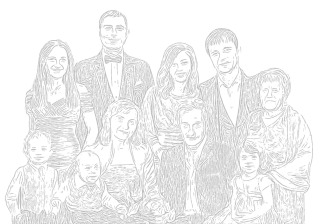
\includegraphics[width=\textwidth]{_cover/to.jpg}
    \emph{Dedicated to my Family}\\
  \end{minipage}
\end{figure}
~
\vspace{2cm}

\noindent The purpose of this book is not merely to instruct but to embark on a shared journey into the realm of 
platform-agnostic application development using Flutter. I've started that book by knowing nothing about Flutter and 
Dart, and the spent time have given me just an initial impulse to the mastery, but I still have something to share with 
you. 

\vspace{3mm}

\noindent I am confident that the time spent on coding (approximately 200 hours) can suffice for grasping the 
fundamental concepts of any programming language or framework, regardless of your prior background, as long as you 
progressively tackle more complex tasks while gradually reducing the need for assistance.

\vspace{3mm}

\noindent My approach to learning has evolved into a day-to-day habit, which I've diligently followed over the past 
20 years while working as a full-stack developer. My technical proficiency is complemented by a profound customer 
focus and business acumen. That possess insights into a product, project, and software life cycles.

\vspace{3mm}

\noindent I warmly invite you to join this project as it unfolds throughout the pages of this book. Together, we will 
embark on an exploration of Flutter and its extensive capabilities. This collaborative learning journey promises to 
be both exciting and enriching as we delve further into the depths of this versatile framework.


\vspace{1cm}

%\texttt{Contributors:}
%Viachaslau Lyskouski, ...

\noindent \emph{\small © Viachaslau Lyskouski, 2023: Creative Commons Attribution-NonCommercial-NoDerivatives 4.0 
International (CC BY-NC-ND 4.0)}
            

\newpage
\thispagestyle{empty}
~

\tableofcontents

%\listoffigures 

%\listoftables 

%\input{./example}
%\markdownInput{./example.md}

\section*{Introduction}
\addcontentsline{toc}{section}{Introduction}
% Copyright 2023 The terCAD team. All rights reserved.
% Use of this content is governed by a CC BY-NC-ND 4.0 license that can be found in the LICENSE file.

Dear readers, I invite you to join me on a journey into a platform-agnostic application development, starting from 
ground zero. Meaning, that we (me and, possibly, you) might know nothing about cross-platform or mobile development, 
\q{Flutter}-framework, \q{Dart}-language, by not having even an idea for the application; ideally, it might 
be chosen a market, which to shake (in our case, -- financial accounting).

That book might be misaligned with the concepts that you're following, respecting, or adepting; by representing the 
author's vision, that's why I invite you to argue with me (\emph{and kindly request your assistance in identifying 
possible errors and misprints}) on the pages of a repository that contains the sources of this book and an application 
that we'll develop together as reading through 
\href{https://github.com/lyskouski/app-finance}{https://github.com/lyskouski/app-finance}. And... 
who knows, may be your arguments will change the ground ideas of that book, and we'll republish it together. 
So, here are those statements:

\begin{itemize}
\setlength{\itemsep}{3pt}
\setlength{\parskip}{0pt}
\setlength{\parsep}{0pt}
    \item Creating any program is similar to a pottery workshop flow, by taking amorphous idea and shaping it. Through 
    the time it can be changed an architectural style (homogeneous, layered, multitier, microservices, etc.), structure 
    (monolithic, distributed, hierarchical, etc.), even platform (from platform specific to serverless), and language. 
    It's all about being Agile, being adaptive to all external and internal challenges. Meaning, that the application's 
    revenue justifies any refactoring, including the possibility of re-creating it from scratch.

    \item Programming is not something about creativity, in its pragmatic meaning (\emph{no one, except the author, 
    will be able to accurately obtain the same result if the same initial situation is created}), but mastery 
    (\emph{how accurate, quick, balanced, and far-sighted will be your implementation}).

    \item Instruments (languages, frameworks, libraries, etc.) should be adapted to solve the problem instead of 
    adapting initial ideas to a capability of available / known tools.

    \item Instead of being \q{I}, \q{T}, \q{U}, or \q{M}-shaped, nowadays dictate us to be \q{\_}-shaped 
    (underscore-shaped). While the most scientists maintain a broad outlook with a narrow specialty (\q{T}-shaped), a 
    significant portion of programmers stand on an unstable foundation. Meaning that technologies are infinitely 
    replacing each other through the time via tick-tock model (characterized by periods of evolution and revolution) 
    and the most effective approach is to continuously expand one's fundamental knowledge (polymathy, \cite{Root09}) 
    by staying acquainted with the technologies in use. 
\end{itemize}

\noindent In case of having any discrepancies with this, the book may cause a rejection; and it's the best time to 
refund. Moreover, it is been started without any knowledge in mobile and cross-platform development, Flutter, Dart, and 
understanding the needs of "financial accounting" market. \q{ChartGPT} was used as a mentor, and \q{Midjourney} --
to generate a few images (including covers of that book), and "shared" some design insights.

Returning to the core themes of the book and the selected technologies, it's evident that businesses aim to embrace 
innovative technologies to optimize their processes and provide outstanding user experiences, all while ensuring 
broad platform compatibility. Not so far, Flutter (\emph{Dec 4th, 2018 -- version 1; May 10th, 2023 -- version 3}) 
has emerged as a popular choice for building high-performance, platform-agnostic (desktop, mobile, web) applications. 
And this book, "\emph{From Nothing to Market with Flutter: Desktop, Mobile, and Web Distribution}", road us to a 
comprehensive journey through the creation of a robust competitive application by using Flutter with 
\q{no-server}-basis (while \q{serverless} is mostly associated with cloud-based infrastructure).

The central objective of this book is to illustrate how to harness the extensive capabilities of Flutter to build a 
comprehensive and feature-rich application. Across the chapters, we will delve into every phase of the application 
development process, starting from conceptualization and culminating in distribution:

\begin{itemize}
    \item Take basics in \q{Dart}-language and \q{Flutter}-framework, and how it enables cross-platform development.

    \item Gain insights into the design principles of an application development. 
    
    \item Go through User Interface and Experience practices to create an intuitive user interface.

    \item Discover how to incorporate essential features into the application with a forecast release planning.

    \item Explore strategies for securely interacting with external systems and ensuring data integrity.

    \item Master techniques for testing (unit, widget, integration, and performance tests) and debugging practices. 

    \item Configure the application distribution across all platforms (Windows, Linux, MacOS, Android, iOS) to their 
    marketplaces, and explore strategies for ongoing maintenance and updates.
\end{itemize}

\noindent So, let's embark on this learning curve journey and keep \q{Flutter}ing.

\newpage
\section{[TBD] Bootcamping Dart and Flutter}
% Copyright 2023 The terCAD team. All rights reserved.
% Use of this content is governed by a CC BY-NC-ND 4.0 license that can be found in the LICENSE file.

\markboth{Bootcamping Flutter}{Bootcamping Flutter}

[TBD]


\subsubsection{Asserting Functions Definition}

By defining functions as arguments for widgets, we can use then as an expectation of functions structure.

\begin{lstlisting}
typedef SetViewFunction = String Function(Currency input);

class CurrencySelector extends StatelessWidget {
  SetViewFunction? setView;

  CurrencySelector({
    Key? key,
    this.setView,
  }) {
    setView ??= setDefaultView;
  }

  String setDefaultView(Currency input) {
    // Default implementation
  }
}
\end{lstlisting}


\subsubsection{Ignoring Function Arguments}

Not required fields are specified slightly different in comparison with classes constructors:

\begin{lstlisting}
void add(String value, [int? id]);
\end{lstlisting}


\subsubsection{Applying Getters and Setters for Class Variables}

By migrating our data structures to class objects it can be used additionally getter and setter for class variables.
That will help us to cover, as an example, `description`-attribute for Budget structures by showing 
`Spent Amount / Total Budget`, and for `details`-attribute - `Left Amount`.

\begin{lstlisting}
class MyClass {
  String _name; // Private variable

  // Getter for name
  String get name => _name;

  // Setter for name
  set name(String value) {
    _name = value;
  }
}

void main() {
  MyClass myObject = MyClass();

  // Using the setter
  myObject.name = 'John';

  // Using the getter
  print(myObject.name); // Output: John
}
\end{lstlisting}

In the example above, the `MyClass`-class has a private variable `\_name`. The getter for `\_name` is defined 
using the get keyword, and the setter is defined using the set keyword. The getter returns the value of 
`\_name`, and the setter sets the value of `\_name` to the provided value. By using that approach we can control 
the access to class variables and perform additional logic or validation when getting or setting their values.

One more question, is how to set `DateTime.now()` inside a constructor as default value, since, by defining it inside
the constructor, an error would be taken: The default value of an optional parameter must be constant.

So, to set a default value for a DateTime variable as the current date and time, we can use the `DateTime.now()` method 
during the initialization of the variable.

\begin{lstlisting}
class MyClass {
    DateTime _createdAt;

    MyClass({DateTime? createdAt})
        : _createdAt = createdAt ?? DateTime.now();

    DateTime get createdAt => _createdAt;
}
\end{lstlisting}


\subsubsection{Using cast to resolve dynamic structures}

Migration our Bills to classes construction has lead to an error on .firstWhere when Account of Budget not found. 
To resolve that we have to cast our getter (otherwise it would be an error: type '() => dynamic' is not a subtype 
of type '(() => BudgetAppData)?' of 'orElse') and add orElse operator as following:

\begin{lstlisting}
  dynamic getByUuid(AppDataType property, String uuid) {
    var scope = (_data[property] as Map)['list'];
    return scope.cast<dynamic>() // cast to cover different types, 
    .firstWhere(
      (item) => item.uuid == uuid,
      orElse: () => null, // Return null if not found
    );
  }
\end{lstlisting}


\subsubsection{Differentiating Map Types}

`HashMap`, as named, provides access to items by their hash in (potentially amortized) constant time.

`SplayTreeMap`' is based on a self-balancing binary tree that allows most single-entry operations in amortized 
logarithmic time.

\begin{lstlisting}
class SummaryAppData {
  // Tree provides improved state on sorting
  final _scope = SplayTreeMap<int, String>();
  // Hash gives us better performance to search by key
  final _hash = HashMap<String, int>();

  SummaryAppData({
    required List<String> list,
  }) {
    this.list = list; // Cover the original property by get/set
  }

  // Return list in reversed order
  List<String> get list => _scope.values.toList().reversed.toList();

  set list(List<String> list) {
    for (int i = 0; i < list.length; i++) {
      add(list[i], i + 1);
    }
  }

  add(String value, [int? id]) {
    // Checking that our UUIDs are unique across the list
    if (_hash.containsKey(value)) {
      _scope.remove(_hash[value]);
      _hash.remove(value);
    }
    // Used to sort the list based on last modification 
    int key = id ?? DateTime.now().millisecondsSinceEpoch;
    _scope[key] = value;
    _hash[value] = key;
  }
}
\end{lstlisting}

\newpage
\section{[TBD] Observing Serverless Computing}
% Copyright 2023 The terCAD team. All rights reserved.
% Use of this content is governed by a CC BY-NC-ND 4.0 license that can be found in the LICENSE file.

\markboth{Observing Serverless Computing}{Observing Serverless Computing}

[TBD]

\newpage
\section{[TBD] Conceptualizing Design for Application}
% Copyright 2023 The terCAD team. All rights reserved.
% Use of this content is governed by a CC BY-NC-ND 4.0 license that can be found in the LICENSE file.

\subsection{Insights into Design Principles}
\markboth{Designing the Financial Accounting Application}{Insights into Design Principles}

In today's fast-paced world, managing personal finances has become increasingly important. Whether it's tracking 
expenses, setting budgets, or monitoring investments, individuals are seeking efficient and intuitive solutions to 
keep their financial lives in order. With the advent of mobile applications, designing a robust financial accounting 
application has become a crucial aspect of providing users with a seamless experience and empowering them to take 
control of their finances.

When it comes to designing a financial accounting application, certain key design principles need to be considered. 

\subsubsection{Simplicity and Intuitiveness}
One of the fundamental principles in designing a financial accounting application is simplicity. The application 
should have a clean and intuitive interface, allowing users to effortlessly navigate through various sections and 
perform tasks. Avoid overwhelming users with unnecessary complexities and focus on providing a streamlined experience 
that caters to their specific financial needs.

\paragraph{Minimalistic Design}
Adopt a minimalistic design approach by keeping the user interface clean and uncluttered. 
Avoid overwhelming users with excessive information or visual elements. Use ample white space, clear typography, 
and a consistent color scheme to create a visually pleasing and organized interface.

\paragraph{Clear Navigation}
Ensure that the application's navigation is intuitive and straightforward. Use clear and 
descriptive labels for navigation elements, such as tabs, menus, and buttons. Organize different sections and 
features logically, making it easy for users to find what they need without confusion or frustration.

\paragraph{Consistent User Flow}
Establish a consistent user flow throughout the application. Users should be able to 
predict how different actions and interactions will unfold based on their previous experiences within the app. 
Consistency in the placement of buttons, menus, and other interactive elements helps users develop a mental model 
of the application's interface.

\paragraph{Task-oriented Design}
Understand the specific tasks and goals of your users when it comes to managing their 
personal finances. Design the application around these tasks, prioritizing the most commonly performed actions. 
Provide clear and easily accessible options for adding transactions, creating budgets, viewing reports, and 
performing other essential financial tasks.

\paragraph{Contextual Help and Guidance}
Incorporate contextual help and guidance within the application to assist users in 
understanding its features and functionalities. Use tooltips, on-screen prompts, and informative messages to 
provide relevant information at the right moment. This helps users make informed decisions and ensures they are 
aware of how to use the application effectively.

\paragraph{Streamlined Data Entry}
Make data entry as effortless as possible. Implement features such as auto-suggestions, 
pre-filled forms, and smart categorization to minimize manual input and reduce the chances of errors. Utilize 
input validation and intelligent defaults to guide users and speed up the data entry process.

\paragraph{Feedback and Confirmation}
Provide visual feedback and confirmation to users when they perform actions or operations 
within the application. This reassures users that their inputs have been registered and processed successfully. 
Use loading indicators, success messages, and error notifications to communicate the status of actions clearly.

\paragraph{User Testing and Iteration}
Conduct user testing and gather feedback during the design and development process. 
Observe how users interact with the application, identify pain points, and refine the design based on their input. 
Iteratively improve the interface to address usability issues and enhance the overall user experience.

\paragraph{Accessibility Considerations}
Ensure that the application is accessible to users with disabilities. Follow 
accessibility guidelines and standards to make the application usable by individuals with visual impairments, 
motor limitations, or other accessibility needs. Provide options for adjusting font sizes, color contrasts, and 
support for screen readers to ensure inclusivity.
\\
\\
Remember, the goal is to create an application that can be easily understood and used by a wide range of users, 
regardless of their level of technical expertise. Strive for simplicity and intuitiveness in every aspect of the 
design, making financial management a seamless and enjoyable experience for your users.


\subsubsection{Clear Information Hierarchy}
A well-designed financial accounting application must establish a clear information hierarchy. Prioritize essential 
financial data such as account balances, transactions, and budgets, ensuring they are easily accessible to users. 
Use visual cues like color coding and icons to guide users' attention and make it easier for them to understand 
their financial status at a glance.

\paragraph{Prioritize Key Financial Information}
Identify the most important financial data that users need to see at a glance. 
This typically includes the current account balances, available funds, total expenses, and income summaries. Place 
this information prominently on the main dashboard or home screen of the application.

\paragraph{Categorize and Group Data}
Organize financial data into logical categories and groups. For example, transactions can 
be grouped by date, account, or type (income or expense). Use clear headings and visual cues, such as dividers or 
section headers, to distinguish different categories. This helps users quickly locate and comprehend specific 
information within the application.

\paragraph{Use Visual Hierarchy Techniques}
Utilize visual hierarchy techniques to guide users' attention and emphasize important 
information. Use larger and bolder fonts, contrasting colors, and appropriate typography to make critical data 
stand out. Highlight important values or trends with visual elements such as icons, charts, or graphs.

\paragraph{Progressive Disclosure}
Implement progressive disclosure to manage complex or detailed financial information. Start 
with a high-level overview of the data and provide options to drill down for more detailed insights. For example, 
show summarized expense categories first and allow users to expand each category to view individual transactions.

\paragraph{Consistent Layout and Organization}
Maintain a consistent layout and organization of information across different 
screens and sections of the application. Users should be able to navigate between screens and find information easily 
without having to relearn the interface. Consistency in the placement of elements such as menus, filters, and search 
bars enhances user familiarity and efficiency.

\paragraph{Filter and Search Functionality}
Enable users to filter and search for specific financial data based on their needs. 
Implement filters by date range, transaction type, account, or category. Incorporate a robust search functionality 
that allows users to find transactions, accounts, or specific financial terms quickly.

\paragraph{Contextual Information}
Provide contextual information and explanations where necessary to help users understand the 
meaning and relevance of different financial terms or calculations. Use tooltips or inline help text to clarify any 
complex concepts or jargon that might be unfamiliar to users.

\paragraph{Clear Labels and Icons}
Use clear and concise labels for different elements within the application. Ensure 
that labels accurately represent the actions or functions they perform. Supplement labels with appropriate icons 
to aid in quick recognition and comprehension.

\paragraph{Gestures and Interactions}
Design intuitive gestures and interactions that enable users to access additional 
information or perform actions effortlessly. For example, swipe gestures to reveal more details about a transaction 
or long-press interactions to access context-specific options.

\paragraph{Responsive Design}
Consider the various screen sizes and orientations that users might utilize. Ensure that the 
application's information hierarchy adapts seamlessly to different screen resolutions and orientations, providing a 
consistent and optimal experience across devices.
\\
\\
By implementing a clear information hierarchy, you empower users to navigate their financial data efficiently and gain 
meaningful insights. A well-structured interface reduces cognitive load, making it easier for users to understand 
their financial status and make informed decisions regarding their personal finances.


\subsubsection{Seamless Onboarding}
The onboarding process sets the stage for user engagement and retention. Design a smooth onboarding experience that 
guides users through the initial setup and familiarizes them with the application's key features. Clearly communicate 
the value proposition and benefits of using the application, helping users understand how it can assist them in 
achieving their financial goals.

\paragraph{Concise Introduction}
Provide a concise and compelling introduction to your financial accounting application. Clearly 
communicate the value proposition and benefits users can expect from using the app. Highlight key features that 
differentiate your app from others in the market, emphasizing how it can help users effectively manage their personal 
finances.

\paragraph{Guided Setup Process}
Design a guided setup process that walks users through the initial steps of getting started with 
the application. Break down the setup process into manageable stages or tasks, presenting one step at a time. Each 
step should be clearly defined and accompanied by explanatory text or visual cues to guide users through the setup.

\paragraph{Personalization Options}
Offer personalization options during the onboarding process. Allow users to 
customize their experience by setting preferences, such as currency format, date format, or language. Personalization 
enhances user engagement and creates a sense of ownership over the app.

\paragraph{Sample Data and Interactive Tutorials}
Consider providing users with sample data or interactive tutorials that 
demonstrate how to use the application effectively. This can help users visualize how their financial information 
will be presented and give them a hands-on experience before entering their own data. Interactive tutorials can 
guide users through key features and actions, ensuring they understand the app's capabilities.

\paragraph{Clear Calls-to-Action}
Use clear and actionable prompts throughout the onboarding process. Provide explicit 
instructions for each step, specifying what users need to do to proceed. Use intuitive buttons or visual cues 
to guide users and make it easy for them to complete each onboarding task.

\paragraph{Progress Indicators}
Incorporate progress indicators to give users a sense of their advancement through the onboarding 
process. This visual feedback assures users that they are making progress and helps manage their expectations regarding 
the remaining steps.

\paragraph{Contextual Help and Tooltips}
Offer contextual help and tooltips at relevant points during the onboarding process. 
Explain unfamiliar terms, provide additional information on features, or clarify any potential confusion. Contextual 
help ensures users feel supported and informed as they navigate through the onboarding experience.

\paragraph{Quick Wins and Rewards}
Include quick wins and rewards during onboarding to motivate and engage users. For example, 
acknowledge and celebrate users' completion of each onboarding task with positive reinforcement messages or small 
virtual rewards. This helps build a positive user experience and encourages users to continue using the app.

\paragraph{Seamless Data Import}
If applicable, provide options for users to seamlessly import their financial data from external 
sources. Enable integration with popular financial institutions, allowing users to connect their bank accounts, credit 
cards, or other financial platforms to automatically import transaction data. Seamless data import saves users time 
and effort, while also demonstrating the value of your app.

\paragraph{Onboarding Feedback}
Gather feedback from users during or at the end of the onboarding process. Offer a way for users 
to provide input, ask questions, or report any issues they may encounter. This feedback can help identify areas for 
improvement and ensure a continuously evolving onboarding experience.
\\
\\
By focusing on creating a seamless onboarding experience, you can effectively introduce users to your financial 
accounting application and help them get started on the right foot. A well-designed onboarding process increases 
user confidence, reduces friction, and sets the stage for long-term engagement and satisfaction.


\subsubsection{Personalization and Customization}
Allow users to personalize their financial accounting experience. Provide options to customize the application's 
theme, layout, and categorization of transactions. Enable users to set financial goals and tailor their budgeting 
preferences according to their unique financial circumstances. Personalization fosters a sense of ownership and 
encourages users to actively engage with the application.

\paragraph{User Profiles}
Implement user profiles that allow individuals to create personalized accounts within the application. User 
profiles can store information such as their name, contact details, and preferred settings. This allows users 
to maintain their personal financial data securely while customizing their experience.

\paragraph{Customizable Dashboards}
Provide users with the ability to customize their dashboard by choosing which financial information and widgets they 
want to see at a glance. Allow users to rearrange widgets, resize them, or add/remove widgets based on their 
priorities. This empowers users to create a personalized dashboard that suits their specific financial tracking needs.

\paragraph{Flexible Categories and Tags}
Allow users to create and customize categories and tags for transactions. Users may have unique income and expense 
categories that align with their specific financial situation or business needs. Giving users the flexibility to 
define and manage their own categories and tags enhances the accuracy and relevance of their financial data.

\paragraph{Budget Customization}
Enable users to set up and customize their budgets based on their financial goals and spending patterns. Provide 
options for users to define budget limits for specific categories, set frequency (monthly, weekly, etc.), and 
allocate funds accordingly. Allow users to adjust their budget over time as their financial circumstances change.

\paragraph{Notification Preferences}
Allow users to personalize their notification preferences. Give them control over which types of financial 
notifications they want to receive, such as transaction alerts, budget warnings, or reminders for bill payments. 
This ensures that users receive relevant and timely notifications without feeling overwhelmed.

\paragraph{Theme and UI Customization}
Provide users with options to personalize the application's theme and user interface. Offer a selection of different 
color schemes, fonts, or layouts that users can choose from. Allowing customization of the app's visual appearance 
enhances user satisfaction and creates a sense of ownership.

\paragraph{Financial Goal Setting}
Incorporate features that allow users to set and track their financial goals. Whether it's saving for a 
vacation, paying off debt, or investing for retirement, users should be able to define their goals within 
the app. Provide progress tracking, reminders, and insights to help users stay motivated and on track towards 
achieving their financial goals.

\paragraph{Data Export and Reports}
Enable users to export their financial data and generate customized reports. Users may want to analyze their 
financial information in external tools or share reports with their financial advisors. Offering export options 
in different formats (such as CSV or PDF) and customizable report templates allows users to tailor the output to 
their specific needs.

\paragraph{Localization and Currency Preferences}
Support multiple languages and currencies to cater to a diverse user base. Allow users to choose their preferred 
language and currency formats within the application. This ensures that users feel comfortable and can easily 
understand and interpret their financial data.

\paragraph{Data Backup and Sync Options}
Provide users with the ability to back up their financial data and sync it across multiple devices. This ensures 
that users can access their financial information seamlessly from various platforms while maintaining data integrity.
\\
\\
By offering personalization and customization features, you empower users to adapt the financial accounting 
application to their unique requirements. This level of customization enhances user engagement, satisfaction, 
and overall user experience, making the app feel tailored to their individual financial journey.


\subsubsection{Secure Data Handling}
Financial data is highly sensitive, and users need assurance that their information is secure. Implement robust 
security measures, such as end-to-end encryption and two-factor authentication, to protect users' personal and 
financial data. Clearly communicate your commitment to data privacy and compliance with industry regulations to 
build trust with your users.

\paragraph{Encryption}
Implement strong encryption techniques to safeguard users' data both in transit and at rest. Utilize 
industry-standard encryption algorithms to encrypt sensitive information such as account credentials, transaction 
details, and personal identifiers. Encryption adds an extra layer of protection and ensures that even if data is 
compromised, it remains unintelligible to unauthorized parties.

\paragraph{User Authentication}
Implement robust user authentication mechanisms to verify the identity of users accessing the 
application. Require strong and unique passwords, and consider implementing multi-factor authentication (MFA) for 
an added layer of security. MFA involves a combination of something the user knows (password), something they have 
(such as a token or mobile device), or something they are (biometrics).

\paragraph{Role-Based Access Control}
Implement role-based access control (RBAC) to restrict access to sensitive data and 
functionalities based on user roles and permissions. Assign different access levels to different user types, 
such as administrators, account holders, or auditors. This helps prevent unauthorized access and ensures that 
users only have access to the data and features relevant to their role.

\paragraph{Regular Security Audits and Updates}
Conduct regular security audits and assessments to identify and address any 
vulnerabilities or weaknesses in the application's infrastructure and codebase. Stay updated with security best 
practices and patches for the technologies and frameworks used in the application. Promptly apply security updates 
and fixes to ensure the application is protected against known vulnerabilities.

\paragraph{Secure Data Transmission}
Ensure that data transmitted between the application and its servers is protected using 
secure protocols such as HTTPS (HTTP over SSL/TLS). HTTPS encrypts data during transmission, preventing unauthorized 
interception or tampering. Avoid transmitting sensitive data via unencrypted channels, such as plain HTTP.

\paragraph{Data Minimization}
Practice data minimization by collecting and storing only the necessary information required for 
the application's functionality. Minimize the collection of sensitive data, and regularly review and purge outdated 
or no longer needed data. This reduces the risk of exposure and potential harm in the event of a data breach.

\paragraph{Secure Storage}
Implement secure storage mechanisms to protect user data within the application's infrastructure. 
Ensure that sensitive data is stored in an encrypted format, whether in databases or cloud storage. Employ secure 
server configurations, access controls, and intrusion detection systems to prevent unauthorized access to stored data.

\paragraph{Regular Backups}
Perform regular backups of user data to prevent data loss in the event of system failures, 
disasters, or other unforeseen circumstances. Store backups in secure locations with restricted access to 
maintain data integrity and availability.

\paragraph{Security Awareness and Training}
Educate your development team and employees about secure coding practices, data 
handling procedures, and the importance of maintaining strong security measures. Regularly train personnel on 
security protocols and potential threats, such as phishing attacks or social engineering techniques.

\paragraph{Privacy Policy and Transparency}
Clearly communicate your application's privacy policy and data handling practices to 
users. Inform them about the types of data collected, how it is used, and who has access to it. Obtain explicit 
consent from users for collecting and processing their data. Be transparent about how you protect user information 
and handle security incidents, providing clear channels for users to report any concerns.
\\
\\
By prioritizing secure data handling practices, you establish trust with users and safeguard their sensitive 
financial information. Proactively addressing security measures helps mitigate risks and provides users with 
the confidence that their personal and financial data is protected within the application.


\subsubsection{Visualizing Financial Data}
Effective data visualization plays a vital role in a financial accounting application. Presenting financial 
information in a visually appealing and understandable manner enhances users' comprehension and enables them 
to make informed financial decisions. Utilize charts, graphs, and interactive dashboards to showcase spending 
patterns, investment performance, and budget progress.

\paragraph{Overview Dashboards}
Create visually appealing and informative overview dashboards that provide users with a high-level summary of their financial information. Use charts, graphs, and key performance indicators (KPIs) to present data such as account balances, income versus expenses, savings progress, or net worth. These visual summaries enable users to quickly assess their financial situation at a glance.

\paragraph{Transaction Visualization}
Represent individual transactions using intuitive and informative visuals. Utilize color-coded icons, symbols, or illustrations to indicate transaction types (income, expense, transfer) or payment methods (cash, credit card). Consider displaying transaction details such as date, category, amount, and account in a concise and visually appealing manner.

\paragraph{Category Breakdown}
Present a breakdown of expenses or income categories through visual charts, such as pie charts, bar graphs, or stacked column charts. This visual representation allows users to identify spending patterns, understand where their money is going, and make adjustments to their budget or financial goals accordingly.

\paragraph{Trend Analysis}
Enable users to analyze financial trends over time using line graphs or area charts. Visualize income, expenses, or 
account balances over a specific period, allowing users to identify patterns, seasonal variations, or anomalies. 
Include interactive features like zooming or panning to allow users to explore data in detail.

\paragraph{Budget Tracking}
Use progress bars, thermometers, or visual indicators to track users' progress toward their budgeting goals. Represent 
the budgeted amount versus actual expenses visually to provide users with a clear understanding of their spending 
habits and help them stay within their financial targets.

\paragraph{Forecasting and Predictive Analytics}
Incorporate forecasting and predictive analytics into visualizations to assist users in planning and decision-making.
Use line charts or trendlines to project future income, expenses, or savings based on historical data. Predictive 
analytics can help users anticipate future financial scenarios and make informed financial choices.

\paragraph{Interactive Filters and Drill-Downs}
Provide interactive filters and drill-down options to allow users to explore financial data from different 
perspectives. Users should be able to filter data based on specific criteria such as time range, category, 
account, or transaction type. Enabling drill-down functionality allows users to delve into detailed information 
by interacting with specific data points or categories.

\paragraph{Comparative Analysis}
Enable users to compare different financial metrics or periods side by side using visualizations like bar charts, 
line graphs, or stacked area charts. This allows users to identify trends, compare performance, or evaluate the 
impact of financial decisions over time.

\paragraph{Heat Maps and Color Schemes}
Utilize heat maps or color schemes to highlight data patterns or variations. For example, use color gradients to 
represent spending intensity, where darker colors indicate higher expenses. Heat maps can help users quickly identify 
areas of focus or anomalies in their financial data.

\paragraph{Interactive Dashboards}
Create interactive dashboards that allow users to customize and personalize their data visualization experience. 
Provide options for users to choose the types of charts, graphs, or visual elements they prefer and arrange them 
on the dashboard according to their preferences. Interactive elements such as tooltips, hover effects, or clickable 
areas can provide additional context and details.
\\
\\
By effectively visualizing financial data, you empower users to understand their financial picture, identify trends, 
and make informed decisions. Well-designed visualizations enhance data comprehension, engagement, and the overall 
user experience, making it easier for users to take control of their finances.


\subsubsection{Seamless Integration with Financial Institutions}
To provide users with a comprehensive financial tracking experience, integrate the application with financial 
institutions and services. Enable users to connect their bank accounts, credit cards, and investment platforms 
to automatically import transaction data. Implement synchronization features to ensure real-time updates and 
seamless reconciliation between the application and external financial sources.

\paragraph{Account Connectivity}
Provide users with a seamless process to connect their financial accounts from various institutions. 
Implement secure and industry-standard protocols such as OAuth or Open Banking APIs to establish a secure connection 
between the application and the financial institution's systems. This allows users to authenticate their accounts 
directly with the financial institution, ensuring their login credentials remain secure.

\paragraph{Multiple Account Types}
Support integration with a wide range of financial accounts, including checking accounts, 
savings accounts, credit cards, investment accounts, and loans. This enables users to centralize their financial 
data and track their transactions, balances, and investments from multiple institutions within a single application.

\paragraph{Transaction Data Import}
Enable users to import their transaction data seamlessly from connected financial institutions. 
Provide options for users to import transactions for specific time periods or select specific accounts for data 
retrieval. Implement efficient data synchronization mechanisms to keep the imported transactions up-to-date, 
ensuring users have the latest financial information at their fingertips.

\paragraph{Transaction Categorization}
Automatically categorize imported transactions based on predefined rules or machine 
learning algorithms. This helps users save time by reducing the manual effort required to categorize each transaction
individually. Additionally, allow users to customize and adjust categorizations as per their preferences.

\paragraph{Balance and Account Updates}
Regularly update account balances and transaction information from connected financial 
institutions. Implement automated processes to fetch and update account balances, ensuring users have real-time 
visibility into their financial standing.

\paragraph{Data Security and Privacy}
Prioritize data security and privacy when integrating with financial institutions. Adhere 
to industry-standard security practices, including encryption, secure data transmission, and compliance with data 
protection regulations such as GDPR or CCPA. Clearly communicate to users how their data is handled, stored, and 
secured within the application.

\paragraph{Error Handling and Notifications}
Implement robust error handling mechanisms to handle potential connectivity issues 
or errors that may occur during the integration process. Notify users of any issues encountered during data retrieval, 
synchronization, or account connectivity. Provide clear instructions on how to resolve the issue or guide users to 
appropriate support channels for assistance.

\paragraph{Reconciliation and Verification}
Offer features to help users reconcile their imported transaction data with their 
bank statements. Enable users to mark transactions as verified or reconciled once they have cross-checked them with 
their official bank statements. This ensures data accuracy and helps users identify any discrepancies or missing 
transactions.

\paragraph{Support for Multiple Financial Institutions}
Support integration with a wide range of financial institutions, including 
banks, credit unions, investment firms, and online payment platforms. Aim to provide comprehensive coverage, allowing 
users to connect with their preferred financial institutions regardless of their location or size.

\paragraph{Continuous Integration Enhancements}
Regularly update and enhance the integration capabilities of the application to 
adapt to evolving financial institution APIs and data formats. Stay informed about industry changes and ensure the 
application remains compatible with the latest standards and protocols.
\\
\\
By achieving seamless integration with financial institutions, users can easily import and manage their financial 
data within the application, providing them with a holistic view of their financial health. This integration streamlines 
the process of tracking transactions, monitoring account balances, and gaining insights into their overall financial 
well-being.


\subsubsection{Cross-Platform Accessibility}
In today's digital landscape, users expect applications to be accessible across multiple devices and platforms. 
Design a financial accounting application that works seamlessly on smartphones, tablets, and desktop computers, 
supporting both iOS and Android platforms. Cross-platform accessibility ensures users can access their financial 
information anytime, anywhere.

\paragraph{Responsive Design}
Implement a responsive design approach to ensure that the application adapts and optimizes its layout and user 
interface based on the screen size and resolution of the device being used. This enables users to access and interact 
with the application smoothly on various devices, including desktops, laptops, tablets, and smartphones.

\paragraph{Native Mobile Apps}
Develop native mobile applications for popular platforms such as iOS and Android. Native apps provide a tailored 
user experience, leveraging the platform-specific features, performance optimizations, and user interface guidelines. 
Native apps can offer enhanced performance, offline capabilities, and seamless integration with device functionalities, 
providing users with a more optimized experience on their respective mobile platforms.

\paragraph{Web-Based Application}
Build a web-based version of the financial accounting application that can be accessed through web browsers on 
different devices. Ensure compatibility across major browsers, including Google Chrome, Mozilla Firefox, Safari, 
and Microsoft Edge. Design the web application to be user-friendly and intuitive, offering a consistent experience 
regardless of the operating system or device.

\paragraph{Cloud Storage and Syncing}
Utilize cloud storage solutions to store user data and ensure seamless syncing across devices. This allows users 
to access their financial information and perform tasks consistently, regardless of the device they are using. 
Implement synchronization mechanisms that automatically update data in real-time, ensuring users have the latest 
information available on all their devices.

\paragraph{Unified User Accounts}
Implement a unified user account system that allows users to access their financial data across multiple platforms 
seamlessly. Users should be able to log in with the same credentials on any device and have their data synced 
automatically. This provides a cohesive experience, ensuring users can seamlessly switch between devices while 
maintaining access to their financial information.

\paragraph{Consistent User Experience}
Strive for a consistent user experience across all platforms and devices. Ensure that the core functionalities, 
features, and navigation patterns remain consistent regardless of the platform or device being used. This allows 
users to familiarize themselves with the application quickly and reduces the learning curve when switching between 
devices.

\paragraph{Device-Specific Features}
Leverage device-specific features and capabilities to enhance the user experience on different platforms. For 
example, on mobile devices, leverage features like camera integration for scanning receipts, push notifications 
for transaction alerts, or biometric authentication for added security and convenience.

\paragraph{Accessibility Standards}
Adhere to accessibility standards and guidelines to ensure that the application is usable by individuals with 
disabilities. Implement features such as adjustable font sizes, high contrast modes, screen reader compatibility, 
and keyboard navigation support. By making the application accessible, you can cater to a wider range of users 
and ensure inclusivity.

\paragraph{User Feedback and Testing}
Regularly gather user feedback and conduct testing on various devices and platforms to identify any compatibility 
or usability issues. Use this feedback to make necessary improvements and optimizations to ensure a seamless 
cross-platform experience.
\\
\\
By focusing on cross-platform accessibility, you enable users to access and use the financial accounting application 
effortlessly across different devices, operating systems, and platforms. This broadens the application's reach, 
enhances user satisfaction, and allows users to manage their finances conveniently, regardless of the devices they 
prefer to use.


\subsubsection{Continuous Improvement and User Feedback}
Designing a financial accounting application is an iterative process. Encourage users to provide feedback and 
actively seek their input to identify areas for improvement. Regularly update the application based on user 
feedback, addressing bug fixes, introducing new features, and enhancing the user experience. This ongoing 
commitment to improvement will foster user loyalty and satisfaction.

\paragraph{User Feedback Channels}
Provide various channels for users to share their feedback, suggestions, and concerns. Offer options such as in-app 
feedback forms, email support, community forums, or social media channels. Make it easy for users to voice their 
opinions and actively encourage them to provide feedback on their experience with the application.

\paragraph{Regular Surveys and Questionnaires}
Conduct periodic surveys or questionnaires to gather insights from users. Ask specific questions about their 
satisfaction level, pain points, desired features, and overall user experience. Use this feedback to identify 
areas for improvement and prioritize development efforts based on user needs and preferences.

\paragraph{User Testing and Usability Studies}
Conduct user testing sessions and usability studies with a diverse group of users. Observe their interactions with 
the application, gather feedback on specific features or workflows, and identify areas where users face challenges 
or confusion. User testing helps uncover usability issues and provides valuable insights for refining the 
application's design and functionality.

\paragraph{Analyze User Behavior}
Utilize analytics tools to track user behavior within the application. Monitor how users navigate through different 
screens, identify drop-off points, and track usage patterns. Analyzing user behavior data helps identify areas that 
require attention and reveals opportunities for enhancing the user experience.

\paragraph{Feature Requests and Prioritization}
Actively listen to user feature requests and suggestions. Maintain a feature request system where users can submit 
and upvote ideas. Regularly review and prioritize feature requests based on their popularity, alignment with the 
application's goals, and potential impact on user satisfaction. Communicate updates on feature requests to keep 
users informed and engaged.

\paragraph{Agile Development Approach}
Implement an agile development approach that allows for iterative development and continuous improvement. Break 
down development tasks into manageable increments and regularly release updates that address user feedback and 
incorporate new features. This iterative approach ensures that user feedback is actively incorporated into the 
development process, leading to a more user-centered application.

\paragraph{Bug Reporting and Issue Resolution}
Provide a seamless process for users to report bugs, issues, or technical glitches they encounter. Ensure that 
reported issues are acknowledged promptly, and transparent communication is maintained throughout the resolution 
process. Regularly release bug fixes and updates to address reported issues and provide users with a stable and 
reliable application.

\paragraph{Release Notes and Communication}
Clearly communicate updates, enhancements, and bug fixes to users through release notes or in-app notifications. 
Explain how the updates address user feedback and improve the application's functionality or user experience. 
Transparent communication demonstrates your commitment to listening to users and continuously improving the 
application.

\paragraph{Beta Testing and Early Access Programs}
Engage enthusiastic users in beta testing or early access programs to gather feedback on upcoming features or 
major updates. Beta testers can provide valuable insights, uncover edge cases, and help identify any issues 
before a wider release. Involve beta testers in the feedback loop and consider their suggestions for further 
enhancements.

\paragraph{Continuous Learning and Adaptation}
Foster a culture of continuous learning and adaptation within your development team. Encourage regular retrospectives 
to reflect on the development process, user feedback, and areas for improvement. Embrace an agile mindset that
embraces change and actively seeks opportunities to iterate and refine the application based on user feedback.
\\
\\
By prioritizing continuous improvement and user feedback, you demonstrate a commitment to delivering an application 
that meets users' needs and expectations. User feedback becomes a valuable source of insights and inspiration for 
enhancing the application's functionality, usability, and overall user experience. This iterative approach ensures 
that the application evolves and remains relevant in a rapidly changing landscape, ultimately leading to increased 
user satisfaction and loyalty.
\\
\\
By incorporating these design principles into your financial accounting application, you can create a powerful 
tool that enables individuals to effectively track and manage their personal finances. Remember, the key is to 
keep the user at the forefront of your design decisions, prioritizing simplicity, security, and usability. 
Empower users with the means to take control of their financial well-being through an intuitive and 
feature-rich application.

\subsubsection{Shake the Market}

One potential "killer feature" that could help the financial accounting application stand out in the market is 
an AI-powered Smart Expense Tracker. Here's how this feature could revolutionize the user experience.

The Smart Expense Tracker leverages artificial intelligence and machine learning algorithms to automate and 
simplify the process of tracking expenses. It offers the following functionalities.

\paragraph{Automated Expense Categorization}
The AI-powered system can automatically categorize expenses based on transaction data, eliminating the need 
for manual categorization. It analyzes transaction descriptions, amounts, and patterns to intelligently assign 
categories such as groceries, transportation, entertainment, bills, and more. Users can save significant time 
and effort in manually categorizing each expense, making expense tracking effortless and accurate.

\paragraph{Receipt Scanning and OCR}
The Smart Expense Tracker incorporates optical character recognition (OCR) technology to scan and extract data 
from receipts. Users can simply take a photo of a receipt, and the application will automatically extract key 
information such as the vendor, date, amount, and items purchased. This eliminates the hassle of manually entering 
receipt details, reduces errors, and ensures precise expense tracking.

\paragraph{Real-time Expense Insights}
The AI-powered system provides real-time insights and analytics on users' spending patterns. It offers visualizations, 
charts, and graphs that highlight monthly spending trends, category breakdowns, and comparisons with previous periods. 
Users can quickly identify areas where they are overspending, set budget goals, and receive personalized 
recommendations for optimizing their finances.

\paragraph{Intelligent Budgeting and Notifications}
The Smart Expense Tracker intelligently analyzes users' income, expenses, and financial goals to create personalized 
budgets. It provides proactive notifications and alerts when users exceed their budget limits or approach predefined 
spending thresholds. These timely notifications help users stay on track, manage their finances effectively, and 
avoid overspending.

\paragraph{Smart Savings Suggestions}
Based on users' spending patterns and financial goals, the application can suggest potential savings opportunities. 
It identifies areas where users can cut costs, offers recommendations for saving money, and highlights opportunities 
for optimizing their budgets. Users receive tailored suggestions that align with their financial objectives, 
empowering them to make informed decisions and improve their financial health.

\paragraph{Predictive Expense Forecasting}
Leveraging historical spending data and machine learning algorithms, the Smart Expense Tracker can forecast future 
expenses with a high degree of accuracy. It provides users with estimated projections of their upcoming expenses, 
allowing them to plan and allocate funds accordingly. This feature enables users to proactively manage their 
finances and make informed decisions based on anticipated expenses.

\paragraph{Integration with Financial Institutions}
The Smart Expense Tracker seamlessly integrates with users' bank accounts and credit cards, automatically importing 
transaction data and keeping it up to date. It provides a comprehensive view of users' financial data in one 
centralized dashboard, offering a holistic perspective on their income, expenses, and financial health.
\\
\\
By incorporating the AI-powered Smart Expense Tracker as a killer feature, the financial accounting application 
can differentiate itself in the market. It simplifies and automates the expense tracking process, delivers actionable 
insights, and empowers users to make smarter financial decisions. This feature not only enhances the user experience 
but also sets the application apart from competitors, potentially capturing a significant market share.


\newpage
\section{[WIP] Implementing Core Functionality}
% Copyright 2023 The terCAD team. All rights reserved.
% Use of this content is governed by a CC BY-NC-ND 4.0 license that can be found in the LICENSE file.

\subsection{Configuring Development Environment}
\markboth{Implementing Core Functionality}{Configuring Development Environment}

Assume, our first steps we're doing from knowing nothing neither about Flutter, nor Dart. So, the better way to start 
from that position is to use some templates (and Flutter kindly provides us such an option).

But, initially, we do need to download and install Flutter (\href{https://flutter.dev}{https://flutter.dev}) by 
following the installation instructions specific to operating system that is used (as an example, for Windows it 
would be needed to register library directory location in the system's \q{PATH}-variable after downloading its sources, 
\cref{img:fs-windows-path}).

\img{first-steps/windows-path-variable}{Windows 10 \q{PATH}-variable location}{img:fs-windows-path}

The choice of a better Integrated Development Environment (IDE) for Flutter development is something negligible, widely
proposed Visual Studio Code, Android Studio, IntelliJ IDEA; but the truth is that nobody cares, what was used (even VIM,
Notepad, or nano), if the work is done. Nonetheless, further discussions in the book would be relevant to Visual 
Studio Code (\href{https://code.visualstudio.com/}{https://code.visualstudio.com/}) usage in "how-to configure IDE" 
examples if nobody minds.

With Visual Studio Code, let's start from Extensions Marketplace usage by installing "Flutter" and "Dart" extensions, 
right after that IDE will ask regarding the Flutter Software Development Kit (SDK) folder (it's the directory where 
the Flutter was installed / downloaded into).

Inside the Flutter SDK folder, we may find a various directories and files, including:

\begin{itemize}
  \item bin -- Flutter command-line tools, such as \q{flutter}, \q{dart}, and other utilities;
  \item cache -- cached files and downloaded packages;
  \item doc -- documentation;
  \item examples -- code examples and sample projects;
  \item packages -- core Flutter packages and dependencies.
\end{itemize}

After those steps, in Visual Studio Code from Command Palette (by pressing [Ctrl + Shift + P], or [Cmd + Shift + P] 
on macOS) will become available "Flutter: New Project"-command, by clicking on which prompt will ask regarding project 
name and location to generate a basic structure. Going farther, let's open the project in IDE and frustrate a minute 
about a wide variety of different scaring files that's been generated. Breathe... we do need only one of them by 
now, that's located in the \q{lib}-directory. File \q{main.dart} is the project's central orbit, the entry point of our 
application.

\begin{lstlisting}
// ./lib/main.dart
import 'package:flutter/material.dart';
// Entry point
void main() {
  runApp(const MyApp());
}
// 'Stateless' means missing any saved states of MyApp
class MyApp extends StatelessWidget {
  // 'super' - parent class, 'key' - widget unique identifier
  const MyApp({super.key}); // Class constructor
  
  // '@override' - replace implementation from parent class
  @override
  Widget build(BuildContext context) { // Returns 'Widget' instance
    return MaterialApp(
      title: 'Flutter Demo',
      // Application theme definition
      theme: ThemeData(
        // Basic color scheme
        colorScheme: ColorScheme.fromSeed(seedColor: Colors.deepPurple),
        // Configuration of Widgets' styles
        useMaterial3: true,
      ),
      // Main page definition
      home: const MyHomePage(title: 'Flutter Demo Home Page'),
    );
  }
}
// 'Stateful' to re-render widget by changed internal states
class MyHomePage extends StatefulWidget {
  // 'required' means that 'title' is a mandatory for constructor on line 25
  const MyHomePage({super.key, required this.title});
  // 'final' - cannot be changed afterwards
  final String title;
  // Wrap an object for a state management
  @override
  _MyHomePageState createState() => _MyHomePageState();
}
// Underscore is a convention for internal classes, methods, and variables
class _MyHomePageState extends State<MyHomePage> {
  int _counter = 0;
  // Internal method to update '_counter' state
  void _incrementCounter() {
    // 'setState' - a special method to save state
    // ... and re-trigger 'build'-method
    setState(() {
      _counter++;
    });
  }
  // Mandatory method for any Widget-based classes
  @override
  Widget build(BuildContext context) {
    return Scaffold(
      appBar: AppBar(
        backgroundColor: Theme.of(context).colorScheme.inversePrimary,
        title: Text(widget.title),
      ),
      body: Center(
        child: Column(
          mainAxisAlignment: MainAxisAlignment.center,
          children: <Widget>[
            // Usage of 'const' is recommended to improve performance
            // ... for any Widget that's not having a dynamic parameters
            const Text(
                'You have pushed the button this many times:',
            ),
            Text(
              '$_counter', // '$' - for a variable interpolation
              style: Theme.of(context).textTheme.headlineMedium,
            ),
          ],
        ),
      ),
      floatingActionButton: FloatingActionButton(
        onPressed: _incrementCounter,
        tooltip: 'Increment',
        child: const Icon(Icons.add),
      ),
    );
  }
}
\end{lstlisting}

Let's see results of a compilation (\cref{img:fs-app}) by triggering \q{flutter run}-command from a terminal of the 
project directory (as an example, for Visual Studio Code by clicking on "View" in the top menu, selecting "Terminal"; 
short key [Ctrl + backtick]). If no emulators are enabled, it may ask to clarify the type of execution.

\img{first-steps/app-template}{First run with autogenerated application}{img:fs-app}

Valuable tip for any development process is to activate a debug mode, that can be done simply by adding \q{--debug} to 
the previous console command (sample, \q{flutter run -d windows --debug} to run project on Windows in debug mode). Then, 
the process is similar to any other programming language: set breakpoints in a code by clicking in IDE on the left 
margin of the desired line, use the command, inspect variables and their states by stepping through the code. Instead of
any debug mode it can be simply used \q{print}-function to plot anything into console. By taking into account that we 
might know exactly nothing about Flutter (and, possibly, any other programming languages), let's return to that 
statement when our application (and we) will become more mature... too early without any business logic on board.

What we can do in addition, is to emulate a real device usage. That's achievable with the Android SDK by downloading 
(\href{https://developer.android.com/studio}{https://developer.android.com/studio}), installing, and going through 
the initial wizard setup (nothing special by now, choose everything by default). One additional step is to create a 
virtual device (\cref{img:fs-android})... a couple of clicks and we're done (\cref{img:fs-create}).

Once we've set up Android SDK and triggered "Start" for the emulator, Flutter will recognize its availability from
an execution \q{flutter run}. Flutter app will be build and launched on the connected Android emulator (or even real 
device, connected via USB; check manuals if needed).\\

\img{first-steps/android-studio}{Android Studio start page}{img:fs-android}
\img{first-steps/android-studio-create}{Android Studio choose and create Emuator}{img:fs-create}

\noindent Let's dive into the coding!
% Copyright 2023 The terCAD team. All rights reserved.
% Use of this content is governed by a CC BY-NC-ND 4.0 license that can be found in the LICENSE file.

\subsection{[TBD] Prototyping Application Skeleton}
\markboth{Implementing Core Functionality}{Prototyping Application Skeleton}

[TBD]

\subsubsection{Creating Widget Tests} \label{widget-tests}

By now we've created some business logic functionality with not so trivial flow. Not to waste the time on checking it
all the time manually after significant changes or refactoring, let's create some tests to check it for us automatically.

Furthermore we've already broken our first test (that's been provided by a Flutter template generation). At the 
beginning it was covering the `Add`-button as an incremental trigger for the shown counter.

\begin{lstlisting}
void main() {
  testWidgets('Counter increments smoke test', (WidgetTester tester) async {
    // Build our app and trigger a frame.
    await tester.pumpWidget(const MyApp());

    // Verify that our counter starts at 0.
    expect(find.text('0'), findsOneWidget);
    expect(find.text('1'), findsNothing);

    // Tap the '+' icon and trigger a frame.
    await tester.tap(find.byIcon(Icons.add));
    await tester.pump();

    // Verify that our counter has incremented.
    expect(find.text('0'), findsNothing);
    expect(find.text('1'), findsOneWidget);
  });
}
\end{lstlisting}

\noindent Let's check that `Add`-button is opening a Widget with a three named tabs.

\begin{lstlisting}
void main() {
  testWidgets('Given Main page When tap on Create Then opened BillAddPage', (WidgetTester tester) async {
    // App initialization
    await tester.pumpWidget(
        // Taken as is from `void main` of `lib/main.dart`-file
        ChangeNotifierProvider(
            create: (_) => AppData(),
            child: const MyApp(),
        )
    );
    // Checking one of the text widgets
    expect(find.text('Goals'), findsOneWidget);
    // Clicking on `Add`-button
    await tester.tap(find.byIcon(Icons.add));
    await tester.pumpAndSettle(); // Waiting till finished render state
    // Asserting icons on our tabs
    expect(find.byIcon(Icons.insert_invitation), findsOneWidget);
    expect(find.byIcon(Icons.money_off), findsOneWidget);
    expect(find.byIcon(Icons.transform), findsOneWidget);
  });
}
\end{lstlisting}

Here we are, by `tab` and `expect` the flow of the whole application can be checked. Such type of tests are named as 
Widget tests that emphasized by specially named `testWidgets`-function.

Initially, it would be better to concentrate mostly on Business Logic than on the draft state of our pages. We'll 
return later to UI/UX, redesign if not dramatically but vastly, and right after that write a reliable 
Test Suite for the Widgets. To check business based calculations it's used `test`-function, and, by example, we would
take our implemented Account Recalculation flow.

\begin{lstlisting}
// test/unit/_classes/data/account_recalculation_test.dart 
void main() {
  // `group` works as a prefix to all the tests inside
  group('Account Recalculation:getDelta', () {
    late AccountRecalculation mock; // Deferred initialization 
    // `setUp` - is going to be executed before each test
    // `setUpAll` - once at the beginning of group evaluation
    setUp(() {
      final accountMock = AccountAppData(
        uuid: '1',
        title: 'test',
        type: AppAccountType.account.toString(),
      );
      mock = AccountRecalculation(
        initial: accountMock.clone(),
        change: accountMock.clone(),
      );
    });
    // Define "table" of input arguments and output assertions
    final testCases = [
      // initial  |   change   | result
      [false, 5.0,  false, 1.0,  -4.0],
      [false, 1.0,  false, 5.0,   4.0],
      [true,  2.0,  false, 3.0,   3.0],
      [false, 2.0,  true,  3.0,  -2.0],
    ];
    // Run all defined Test Cases
    for (var v in testCases) {
      test('initial(hidden[${v[0]}], details[${v[1]}]), change(hidden[${v[2]}], details[${v[3]}]) => ${v[4]}', () {
        // Update inputs
        mock.initial!.hidden = v[0] as bool;
        mock.initial!.details = v[1] as double;
        mock.change.hidden = v[2] as bool;
        mock.change.details = v[3] as double;
        // Assert `AccountRecalculation.getDelta`-method results
        expect(mock.getDelta(), v[4]); 
      });
    }
  });
}
\end{lstlisting}

By typing `flutter test` in the command line we would see something like that:

\begin{lstlisting}
[V] Given Main page When tap on Create Then opened BillAddPage
[V] Account Recalculation:getDelta initial(hidden[false], details[5.0]), change(hidden[false], details[1.0]) => -4.0
[V] Account Recalculation:getDelta initial(hidden[false], details[1.0]), change(hidden[false], details[5.0]) => 4.0
Expected: <3.0>
  Actual: <1.0>
[X] Account Recalculation:getDelta initial(hidden[true], details[2.0]), change(hidden[false], details[3.0]) => 3.0
[V] Account Recalculation:getDelta initial(hidden[false], details[2.0]), change(hidden[true], details[3.0]) => -2.0
Null check operator used on a null value
[X] Account Recalculation:getDelta initial(null), change(hidden[false], details[2.0]) => 2.0
Exited (1)
\end{lstlisting}

\noindent That test has highlighted a dozen of troubles and failures in our code, so, it definitely has not been 
written in vain.

\begin{lstlisting}[firstnumber=17]
// ./lib/_classes/data/account_recalculation.dart
double getDelta() {
  return change.hidden
\end{lstlisting}
{
\xpretocmd{\lstlisting}{\vspace{-12pt}}{}{}
\begin{lstlisting}[firstnumber=20, backgroundcolor=\color{backred}]
(*@\kdiff{-}@*)  ? -initial!.details
\end{lstlisting}
\begin{lstlisting}[firstnumber=20, backgroundcolor=\color{backgreen}]
(*@\kdiff{+}@*)  ? -(initial?.details ?? 0.0)
\end{lstlisting}
\begin{lstlisting}[firstnumber=21, backgroundcolor=\color{backred}]
(*@\kdiff{-}@*)  : change.details - initial!.details;
\end{lstlisting}
\begin{lstlisting}[firstnumber=21, backgroundcolor=\color{backgreen}]
(*@\kdiff{+}@*)  : (initial?.hidden ?? true
(*@\kdiff{+}@*)      ? change.details
(*@\kdiff{+}@*)      : change.details - initial?.details);
\end{lstlisting}
\begin{lstlisting}[firstnumber=24]
}
\end{lstlisting}
}

\subsubsection{Creating Automated Quality Gates}

Tests writing is not enough for a quality check, we have to implement some dozen of automation till the phase 
when will become too lazy to trigger that manually. In addition, Flutter provides a couple of commands for the 
code improvement:
\begin{lstlisting}
flutter analyze // Static analysis of Dart code
dart format // Apply rules from https://dart.dev/effective-dart/style#formatting
dart fix // Check what can be improved, by `--apply` will change the code
\end{lstlisting}


\paragraph{Creating Git Hooks}

Someone might think that additional checks before `git commit` and `git push` will slowdown the development process, 
contrary that minimizes pushes back and forward to resolve failures on CI/CD build procedure. For a really big projects
that might take hours in contrast with seconds on local environment. Surely, the automation process has to be done
accurately and properly, otherwise it will be constantly bored.

Implementing git hooks is a preparation of bash-scripts for execution, so, let's discuss here `pre-push`-file (since
`pre-commit`-file contains almost the same logic for another scope of commands).

\begin{lstlisting}[language=bash]
#!/bin/bash

status=0

flutter test # Trigger tests
status_test=$? # Take status for lastly executed command

if [ $status_test -ne 0 ]; then
  echo "[x] flutter test - failed."
  status=1
else
  echo "[+] flutter test - passed."
fi

exit $status
\end{lstlisting}

\noindent Let's use Grinder to install our hooks (`dart run grinder:init` can be used to generate a skeleton 
structure if it's missing yet).

\begin{lstlisting}
// ./tool/grind.dart
import 'dart:io';
import 'package:path/path.dart' as path;
import 'package:grinder/grinder.dart';

main(args) => grind(args);

@Task('Install Git Hooks')
installGitHooks() {
  final currDir = Directory('./');
  final hookDir = Directory('./.git/hooks');
  final hookNames = ['pre-commit', 'pre-push'];
  for (final name in hookNames) {
    log('Applying: $name');
    final sourceFile = File(path.join(currDir.absolute.path, name));
    sourceFile.copySync(path.join(hookDir.absolute.path, name));
  }
  log('Git Hooks applied!');
}
\end{lstlisting}

\noindent After that by using command line, let's check what we have:

\begin{lstlisting}[language=bash]
$ dart run grinder -h
Dart workflows, automated.

Usage: grinder [options] [<tasks>...]

Global options:
  --no-color           Whether to use terminal colors.
  --version            Reports the version of this tool.
  -h, --help           Print this usage information.

Available tasks:
  install-git-hooks    Install Git Hooks
  sort-translations    Update Translations by sorting values alphabetically

$ dart run grinder install-git-hooks
  grinder running install-git-hooks
  
  install-git-hooks
    Applying: pre-commit
    Applying: pre-push
    Git Hooks applied!
  
  finished in 0.0 seconds

$ git add .
$ git commit -m "Sample Commit"
Computing fixes in app-finance (dry run)...
Nothing to fix!
Formatted 56 files (0 changed) in 0.42 seconds.

[+] dart fix - passed.
[+] dart format - passed.
[+] dart run grinder sort-translations - passed.
Sample Commit
 3 files changed, 65 insertions(+), 90 deletions(-)

$ git push
# ... logs from tests
[+] flutter test - passed.
# ... other logs from git
\end{lstlisting}


\paragraph{Adding Grinder Helpers}

We haven't yet discussed our `grinder sort-translations` that was shown through the logs above. That task is needed
to automatically rearrange our labels in `/lib/l10n/app\_*.arb`-files. We might extend our grinder tasks lately
by also checking consistency (enter missing labels across the `.arb`-files), exporting labels to `.scv`-file
for translation purposes, and importing them back.

\begin{lstlisting}
// ./tool/grind.dart
import './localization.dart' as locale;

@Task('Update Translations by sorting values alphabetically')
sortTranslations() {
  // Get all additional arguments for the command
  TaskArgs args = context.invocation.arguments;
  // Run: dart run grinder sort-translations --quiet
  bool isQuiet = args.getFlag('quiet'); // Returns `true` if set
  bool isChanged = locale.sortArbKeys('./lib/l10n');
  if (isChanged && !isQuiet) {
    fail('Changes detected'); // (!) to handle failure
  }
}
\end{lstlisting}

\begin{lstlisting}
// ./tool/localization.dart
import 'dart:convert';
import 'dart:io';
import 'package:grinder/grinder.dart';

bool sortArbKeys(String path) {
  log('Checking $path'); // Add to console output the text
  final arbDir = Directory(path);
  bool isChanged = false;
  // Check, that folder is not missing
  if (!arbDir.existsSync()) {
    log('Error: Directory not found');
    return true;
  }
  // Loop per each file there
  for (var file in arbDir.listSync()) {
    // Take only .arb-files
    if (file is File && file.path.endsWith('.arb')) {
      log('- ${file.path}');
      // `|=` is a boolean OR assignment
      isChanged |= sortArbFileKeys(file);
    }
  }
  log(isChanged ? 'Labels reordered' : 'Nothing was changed');
  return isChanged;
}

bool sortArbFileKeys(File file) {
  // Load data from file
  final jsonContent = file.readAsStringSync();
  final arbMap = json.decode(jsonContent) as Map<String, dynamic>;
  // Sort labels
  final entries = arbMap.entries.toList();
  entries.sort((a, b) {
    final aKey = a.key.startsWith('@') ? a.key.substring(1) : a.key;
    final bKey = b.key.startsWith('@') ? b.key.substring(1) : b.key;
    return aKey.compareTo(bKey);
  });
  final sortedArbMap = Map.fromEntries(entries);
  // Write back to the file with preserved indentation
  const encoder = JsonEncoder.withIndent('    ');
  var jsonOutputContent = encoder.convert(sortedArbMap);
  file.writeAsStringSync(jsonOutputContent);
  return jsonOutputContent != jsonContent; // Check if changed
}
\end{lstlisting}


\paragraph{Activating GitHub Workflow}

We've done with our automation for local environment, let's go further and define quality gates on GitHub repository.

\begin{lstlisting}[language=yaml]
# ./.github/workflows/dart.yml
name: Flutter/Dart Quality Gates # Name that would be shown in Actions tab

on:
  push: # Trigger after a merge
    branches: [ "main" ] # limit to main-branch
  pull_request: # Trigger on pull-request
    branches: [ "main" ] # if the target is main-branch

jobs:
  build:
    runs-on: ubuntu-latest # Environment for execution

    steps:
      - uses: actions/checkout@v3 # Checkout from repository
      - uses: subosito/flutter-action@v2 # Install Flutter/Dart
        with:
          channel: 'stable'
      - run: flutter --version # Show version in logs

      - name: Install Dependencies
        run: flutter pub get

      - name: Verify Formatting
        run: dart format --output=none --set-exit-if-changed .

      - name: Check Localizations ordering
        run: dart run grinder sort-translations

      # Consider passing '--fatal-infos' for slightly stricter analysis.
      - name: Analyze Project Source
        run: flutter analyze

      - name: Run tests
        run: flutter test
\end{lstlisting}

\noindent By preparing a pull-request we would see next representative validations flow 
(\cref{img:pt-github}, \cref{img:pt-github-details})):

\img{prototyping/github-check}{GitHub Toolbar on pull-request}{img:pt-github}

\img{prototyping/github-check-details}{GitHub Workflow Actions details}{img:pt-github-details}

In which way we can improve the current state is to gratitude ourselves by Badges of Workflow Status and Code Coverage.

\begin{lstlisting}[language=bash]
# ./README.md
# Notation of an image with tooltip "Build Status" 
![Build Status](https://github.com/{user}/{repo}/actions/workflows/{workflow-name}.yml/badge.svg?branch=main)
# Notation of an image with a link to our repository
[![Tests Coverage](https://{user}.github.io/{repo}/coverage_badge.svg)](https://github.com/{user}/{repo})
\end{lstlisting}

`Build Status` is supported out of the box (OOTB) by GitHub, just it's needed to replace `\{user\}` (account name
on GitHub), `\{repo\}` (repository name), and `\{workflow-name\}` (name of the file in `.github/workflows`-folder).

`Test Coverage` is needed to be cooked (there are many ways to do that and none of them is universal), and we're 
starting from creating `gh-pages` for our repository (drop hooks from `.git/hooks`-folder if they've been enabled):

\begin{lstlisting}[language=bash]
git switch --orphan gh-pages
git commit --allow-empty -m "Initial commit"
git push -u origin gh-pages
git checkout main
\end{lstlisting}

\noindent That will create for us a special branch that is accessible via \`https://\{user\}.github.io/\{repo\}\`-link. 
Then we need to extend our GitHub Workflow by including there a section to upload artifacts:

\begin{lstlisting}[language=yaml]
# ./.github/workflows/dart.yml
# Updating previously created step by a conditional execution
- name: Run tests
run: |
  if [[ "${{ github.ref }}" == "refs/heads/main" ]]; then
    flutter test --coverage
    dart run grinder coverage-badge # New Grinder task to generate `.svg'-file with coverage
  else
    flutter test
  fi
# New section to upload artifacts
- name: Update Coverage Badge
  # Get default branch variable and compare with current
  if: github.ref == format('refs/heads/{0}', github.event.repository.default_branch)
  uses: peaceiris/actions-gh-pages@v3 # Special action to upload artifacts
  with:
    github_token: ${{ secrets.GITHUB_TOKEN }} # Generated automatically by GitHub
    publish_dir: ./coverage # Folder to upload
\end{lstlisting}

\img{prototyping/badges}{Generated README.md for the repository}{img:pt-badge}

Everything is done (\cref{img:pt-badge})... almost. Coverage 46\% is unbelievable for written tests. The problem is 
that untouched (by tests) files are not included into the report. And, additionally, widget tests cover most of the 
files without checking them. So, let's separate type of tests' execution, and provide additional Grinder task to 
touch all our files for the coverage report.

\begin{lstlisting}[language=yaml]
# ./.github/workflows/dart.yml
- name: Run tests
  run: |
    if [[ "${{ github.ref }}" == "refs/heads/main" ]]; then
      dart run grinder full-coverage
      flutter test --coverage test/unit
      flutter test test/widget
      dart run grinder coverage-badge
    else
      flutter test
    fi
\end{lstlisting}

\begin{lstlisting}
// ./tool/coverage.dart
import 'dart:io';
void scanDirectory(Directory directory, List<String> files) {
  directory.listSync(recursive: true).forEach((entity) {
    if (entity is File && // Check that it's a file
        entity.path.endsWith('.dart') && // Include only Dart
        !entity.path.endsWith('.g.dart')) { // Code generation
      files.add(entity.absolute.path
        .replaceAll(root.absolute.path, '') // Cut out root prefix
        .replaceAll('\\', '/')); // Fix for Windows' systems
    } else if (entity is Directory) {
      scanDirectory(entity, files); // Recursively scan further
    }
  });
}
\end{lstlisting}

\begin{lstlisting}
// ./tool/grind.dart
import './coverage.dart' as coverage;
@Task('Generate file with all lib/**.dart-files included')
fullCoverage() {
  List<String> files = [];
  String content = "// AUTOGENERATED BY `dart run grinder full-coverage` \n";
  final rootFolder = Directory('${Directory.current.path}/lib');
  coverage.scanDirectory(rootFolder, rootFolder, files);
  for (var file in files) {
    content += "import 'package:app_finance$file';\n";
  }
  content += "void main() {}\n";
  File(path.join(Directory.current.path, 'test/_coverage.dart')).writeAsStringSync(content);
}
\end{lstlisting}

\begin{lstlisting}[language=bash]
# .gitignore
# Coverage report
coverage/
test/_coverage.dart
\end{lstlisting}

\noindent 10\% Coverage... here we are. Slowly and progressively, we will correct this assessment but not immediately.
Do remember that we're on an early stage and nothing is neither stable, nor finalized yet.


\subsubsection{Creating Unit Tests with Wrappers (Code Generators)} \label{ut-code-generator}

We've implemented earlier the test for a simple function that is isolated by itself from all other functionality. 
In most of the cases our functions are calling other functions, while unit test has to check the logic of the defined 
function isolately by cutting all external interactions (idealy, even within one class). To achieve that we might
use `Mockito` (\href{https://github.com/dart-lang/mockito}{https://github.com/dart-lang/mockito}):

\begin{lstlisting}
// ./test/unit/_classes/data/account_recalculation_test.dart
// Original class that we're testing
import 'package:app_finance/_classes/data/account_recalculation.dart';
// Wrapping our class by Mockito
@GenerateNiceMocks([MockSpec<AccountRecalculation>()])
import 'account_recalculation_test.mocks.dart';

void main() {
  group('AccountRecalculation updateGoals', () {
    late List<GoalAppData> goals;
    // Data initialization
    setUp(() {
      goals = [
        GoalAppData(title: '1', details: 25.0, progress: 0.0),
        GoalAppData(title: '2', details: 50.0, progress: 0.0),
        GoalAppData(title: '3', details: 100.0, progress: 0.0),
      ];
    });
    // Test Suite (Behavioral Matrix)
    final testCases = [
      (getDelta: 0.0, progress: [0.0, 0.0, 0.0], result: [0.0, 0.0, 0.0]),
      // ... other cases
    ];
    // Loop across all Test Cases
    for (var v in testCases) {
      test('$v', () {// Make test representation named by its inputs
        final mock = MockAccountRecalculation();
        // Wrap "external" method
        when(mock.getDelta()).thenReturn(v.getDelta);
        // Preparing data for the test
        for (int i = 0; i < v.progress.length; i++) {
          goals[i].progress = v.progress[i];
        }
        mock.updateGoals(goals);
        // Asserting results
        for (int i = 0; i < v.result.length; i++) {
          expect(goals[i].progress, v.result[i]);
        }
      });
    }
  });
}
\end{lstlisting}

Almost done... failing since `account\_recalculation\_test.mocks.dart`-file is missing. To resolve that we have to use 
additional a library `build\_runner` (`flutter pub add build\_runner --dev`) that will generate `*.mocks.dart`-files
for us. But that makes our work harder since before each `flutter test` we have to run `flutter run build\_runner build`.
Let's cover that by additional Grinder task:

\begin{lstlisting}
// ./tool/grind.dart
@Task('Generate Mocks')
mock() {
  ProcessResult build = Process.runSync('dart', [
    'run',
    'build_runner',
    'build',
    '--delete-conflicting-outputs',
  ]);
  if (build.exitCode > 0) {
    fail(build.stderr);
  }
}

@Task('Run tests')
@Depends(mock)
test() {
  TaskArgs args = context.invocation.arguments;
  ProcessResult test = Process.runSync(
    'flutter', 
    [
      'test',
      args.getFlag('coverage') ? '--coverage' : '',
      args.getOption('path') ?? ''
    ].where((e) => e != '').toList(), // Drop empty arguments 
    runInShell: true // Otherwise, error: The system cannot find the file specified. 
  );
  if (test.exitCode > 0) {
    fail(test.stderr);
  }
  log(test.stdout);
}
\end{lstlisting}

\begin{lstlisting}[language=bash]
> dart run grinder test
grinder running test

test
  [INFO] Generating build script...
  ...
  [INFO] Succeeded after 51ms with 0 outputs (0 actions)

  00:00 +0: AccountRecalculation updateGoals (getDelta: 0.0, ...
  ...
  00:01 +7: All tests passed!
\end{lstlisting}

\noindent The first test with mocks is passing, but not actually evaluate the original method as we might expect, 
everything is mocked! To achieve a capability of a partial mocking we would need to implement a wrapper around the 
original class. By using `mockGetDelta`-method it would be possible to override (mock) behavior of any method. 

\begin{lstlisting}
class WrapperAccountRecalculation extends AccountRecalculation {
  double Function()? _getDelta;
  // ignore: non_constant_identifier_names
  set mockGetDelta(double Function() value) {
    _getDelta = value;
  }

  @override
  double getDelta() => (_getDelta ?? super.getDelta)();
}
\end{lstlisting}

\noindent So, let's automated that part as well by using the `source\_gen` package, which provides capabilities to 
generate `.dart`-files based on annotations. Firstly, it's needed to register our custom builder via `build.yaml`-file:

\begin{lstlisting}[language=yaml]
# Force to activate our generator
targets:
  $default:
    builders: 
      # Combination of application name and builder definition
      app_finance|wrapper_generator:
        enabled: true # Activate its usage

builders:
  wrapper_generator: # Builder name
    # Builder file location
    import: "package:app_finance/_classes/gen/wrapper_generator.dart"
    # Method name that is used as a factory
    builder_factories: ["wrapperGenerator"]
    build_extensions: {".dart": [".wrapper.dart"]}
    auto_apply: dependents
    build_to: source # Generate to file
    applies_builders: ["source_gen|combining_builder"]
\end{lstlisting}

\begin{lstlisting}
// ./lib/_classes/gen/generate_with_method_setters.dart
class GenerateWithMethodSetters {
  final List<Type> classes;
  const GenerateWithMethodSetters([this.classes = const []]);
}(*@ \stopnumber @*)

// ./lib/_classes/gen/wrapper_generator.dart
Builder wrapperGenerator(BuilderOptions options) => LibraryBuilder(
      WrapperGenerator(),
      generatedExtension: '.wrapper.dart',
    );

class WrapperGenerator extends Generator {
  String build(Iterable<DartObject> annotations) {
    final result = StringBuffer();
    for (final annotation in annotations) {
      final classes = annotation.getField('classes');
      if (classes!.isNull) {
        break;
      }
      for (final name in classes.toListValue()!) {
        final type = name.toTypeValue();
        final classElement = type?.element as ClassElement;
        final visitor = WrapperVisitor(classElement);
        result.writeln(visitor.toString());
      }
    }
    return result.toString();
  }

  @override
  String generate(LibraryReader library, BuildStep buildStep) {
    final result = StringBuffer();
    for (final element in library.allElements) {
      final annotations =
          const TypeChecker.fromRuntime(GenerateWithMethodSetters)
              .annotationsOf(element);
      if (annotations.isNotEmpty) {
        result.writeln(build(annotations));
      }
    }
    return result.toString();
  }
}(*@ \stopnumber @*)
  
// ./lib/_classes/gen/wrapper_visitor.dart
class WrapperVisitor {
  StringBuffer buffer = StringBuffer();
  ClassElement element;

  WrapperVisitor(this.element);

  void addImports() {
    final mainClass = element.enclosingElement.library;
    addImport(mainClass);
    for (final cls in mainClass.importedLibraries) {
      addImport(cls);
    }
    buffer.writeln('');
  }

  void addImport(LibraryElement className) {
    buffer.writeln('// ignore: unused_import');
    buffer.writeln("import '${className.source.uri}';");
  }

  void addClassDefinition() {
    buffer.writeln('class Wrapper${element.name} extends ${element.name} {');
    final constructor = element.unnamedConstructor;
    if (!constructor!.isDefaultConstructor) {
      final properties = constructor.parameters;
      buffer.writeln('  Wrapper${element.name}({');
      if (properties.isNotEmpty) {
        for (var e in properties) {
          buffer.writeln(
              '    ${e.isRequired ? 'required ' : ''}super.${e.name},');
        }
      }
      buffer.writeln('  });');
    }
  }

  void addMethods() {
    for (final m in element.methods) {
      final args = m.parameters.map((e) => e.name).toList().join(', ');
      final name = 'mock${m.name[0].toUpperCase()}${m.name.substring(1)}';
      buffer.writeln('');
      buffer.writeln('  ${m.returnType} Function()? _${m.name};');
      buffer.writeln('  // ignore: non_constant_identifier_names');
      buffer.writeln('  set $name(${m.returnType} Function() value) {');
      buffer.writeln('    _${m.name} = value;');
      buffer.writeln('  }');
      buffer.writeln('');
      buffer.writeln('  @override');
      buffer.writeln('  $m => (_${m.name} ?? super.${m.name})($args);');
    }
  }

  void finalize() {
    buffer.writeln('}');
  }

  @override
  String toString() {
    addImports();
    addClassDefinition();
    addMethods();
    finalize();
    return buffer.toString();
  }
}
\end{lstlisting}

\noindent And, finally, or test would be adjusted to support implemented wrapper:

\begin{lstlisting}
@GenerateNiceMocks([MockSpec<AccountRecalculation>()])
import 'account_recalculation_test.mocks.dart';
@GenerateWithMethodSetters([AccountRecalculation])
import 'account_recalculation_test.wrapper.dart';

test('Demo', () {
  final mock = MockAccountRecalculation();
  final wrapper = WrapperAccountRecalculation();
  when(mock.getDelta()).thenReturn(v.getDelta);
  wrapper.mockGetDelta = mock.getDelta;
  for (int i = 0; i < v.progress.length; i++) {
    goals[i].progress = v.progress[i];
  }
  wrapper.updateGoals(goals);
  verify(mock.getDelta()).called(1);
  for (int i = 0; i < v.result.length; i++) {
    expect(goals[i].progress, v.result[i]);
  }
});
\end{lstlisting}


\subsubsection{Introducing Behavioral Tests (Gherkin)}

Improvement cycles are never ends. Previously (\ref{widget-tests}), we've discussed approach to test widgets and used 
`When ... Given ... Then ...`-notation. That notation is a part of Behavior-Driven Development (BDD), the process
of approaching the desired outcome on first place before the code. But we've used that notation as a comment that is 
useless without any interpreter (since it can be written one flow but tested totally different things; or, it's been 
forgotten to update the comment).

Cucumber (\href{https://docs.cucumber.io}{https://docs.cucumber.io}) is a practical standard, by being widely used, 
a testing framework for Behavior Driven Development.

Gherkin (\href{https://pub.dev/packages/gherkin}{https://pub.dev/packages/gherkin}), as a fully featured parser and 
test runner for Flutter and Dart, would be used by us to convert When/Given/Then(And/But) into a real test steps.

In Cucumber-JVM (as well as in Gherkin) calling steps from step definitions is not supported; this is by design. That's
why I do love Robot Framework (\href{https://robotframework.org}{https://robotframework.org}) that allows to create 
high-level scenarios by combining low-level steps. That limitation "by design" is made to not create a mess, with an 
assumption, that this may lead to an explosion of step definitions, code duplication, and high maintenance costs. We 
won't argue with highly-qualified specialists and take all the risks to our own. Testing is a variation of an art where 
a common sense is a mantra to succeed.

After adding it (`flutter pub add flutter\_gherkin --dev`) into our application, we can start from creation 
`.feature`-file to describe our scenario.

\begin{lstlisting}[language=cucumber]
@account @currency
Feature: Verify Account functionality alignment with expectations

  Scenario: Opened Account Form
    Given I am on "Main" page
    When I tap "Account" header
    And I tap "Create" button
    Then I can see "Account Form" component

  Scenario Outline: Created different Account types
    Given Opened Account Form
    When I fill the "Account" field with <type>
    Then I should see <fields> fields
    But not <hidden> fields

    Examples: 
      | type | fields | hidden |
      | ...  |  ...   |  ...   |
\end{lstlisting}

We've created Scenario "Opened Account Form" and by braking all the recommendations re-used it in Scenario Outline 
for `Given`-step. What's that giving us? To answer that question, let's check how a billing flow might look like:

\begin{lstlisting}[language=cucumber]
  Scenario Outline: Added different Expenses
    Given Created different Account types
    And Created different Budget types
    And Opened Expense Form
    When I fill the "Amount" field with <type>
    ...
    And I tap "Create" button
    Then I should see "Account <account>" deduction by <amount>
    And I should see "Budget <budget>" percentage change to <percent> with left <budget_amount>
\end{lstlisting}

So powerful simplification cannot be ignored, it's not a mess but extreme code-reusability and simplification. If
something would be changed (pipeline to open form, properties, widgets, etc.), a single scenario would be responsible 
for that. The only convention: scenario is written in past tense, step - in present. By following such a simple rule it 
would be always obvious the nested structure. 

Another drawback is that Gherkin runs User Interface tests (mostly known as Selenium tests) by compiling and running 
the original application with enabled Flutter Driver Extension that simulates user behavior. It's not something that we 
might be interested in by now, expecting their fast evaluation via simulation as it's done for widget tests. So, we're 
going to take an interpreter of `.feature`-files and use `flutter\_test`-package for all other stuff. Additional benefit
from that is that a basic Test Terminal in IDE would work for us with all features enabled (to run/re-run a single, a 
group or all tests) and we would still have a single entry point to evaluate all our tests.

But let's proceed iteratively, and implement wrapper around Gherkin to parse `.feature`-files and evaluate 
them (\cref{img:p-bdd}):

\begin{lstlisting}
./test/e2e/e2e_test.dart
void main() {
  // Taking all our .feature files
  late Iterable<File> scope = Directory('./test/e2e')
      .listSync(recursive: true)
      .where((entity) => entity is File && entity.path.endsWith('.feature'))
      .cast<File>();

  group('Behavioral Tests', () {
    for (var file in scope) {
      testWidgets(file.path, (WidgetTester tester) async {   
        await tester.pumpWidget(ChangeNotifierProvider(
          create: (_) => AppData(),
          child: const MyApp(),
        ));
        final runner = FileRunner(file);
        await runner.init(tester);
        expect(await runner.run(), true);
      });
    }
  });
}(*@ \stopnumber @*)

// ./test/e2e/_steps/file_runner.dart
class FileRunner {
  File file;
  final language = LanguageService();
  final parser = GherkinParser();
  final featureFile = FeatureFile(RunnableDebugInformation.EMPTY());
  late FeatureFileRunner runner;
  static late WidgetTester tester;

  FileRunner(this.file) {
    language.initialise();
    runner = FeatureFileRunner(
      FlutterTestConfiguration(),
      TagExpressionEvaluator(),
      ExecutableStepIterator().aggregate(),
      ProgressReporter(),
      AggregatedHook(),
    );
  }

  Future<void> init(WidgetTester tester) async {
    FileRunner.tester = tester;
    // Parsing taken file by Gherkin
    final parserResult = await parser.parseFeatureFile(
      file.readAsStringSync(),
      '',
      ProgressReporter(),
      language,
    );
    for (final feature in parserResult.features) {
      featureFile.addChild(feature);
    }
  }

  Future<bool> run() async {
    return await runner.run(featureFile);
  }
}(*@ \stopnumber @*)

// ./test/e2e/_steps/executable_step_iterator.dart
class ExecutableStepIterator {
  final List<CustomParameter> param = <CustomParameter>[];

  ExecutableStepIterator() {
    param.addAll([
      NumParameterLower(),
      IntParameterLower(),
      StringParameterLower(),
      WordParameterLower(),
    ]);
  }

  List<ExecutableStep> _register(List<dynamic> steps) {
    return steps.map(
      (s) => ExecutableStep(GherkinExpression(s.pattern, param), s),
    ).toList();
  }

  Iterable<ExecutableStep> aggregate() {
    return _register([
      OnDefinedPage(),
      TapDefinedButton(),
      TapDefinedHeader(),
      CanSeeDefinedComponent(),
    ]);
  }
}(*@ \stopnumber @*)

// ./test/e2e/_steps/given/on_defined_page.dart
class OnDefinedPage extends Given1<String> {
  @override
  RegExp get pattern => RegExp(r"I am on {string} page");

  @override
  Future<void> executeStep(String route) async {
    // ... test step implementation
  }
}(*@ \stopnumber @*)

// ... other classes implementation: TapDefinedButton, TapDefinedHeader, CanSeeDefinedComponent
\end{lstlisting}

\img{prototyping/bdd-test}{Behavioral Test evaluation}{img:p-bdd}

What can be noticed, is that we have to declare all our implementations (Given/When/Then) as a list of classes. 
That stuff is better to be automated by scanning `\_steps`-folder and adding all classes into the list, and we do 
know already (\ref{ut-code-generator}) how to achieve that.

Additional convention should be taken into account; as soon as we using Scenario as a low-level step, it should be
excluded from an execution scope. Let's move such scenarios into `.resource`-files and cover them by generics 
(additional code generated classes per each scenario in `.resource`-files).

\begin{lstlisting}
// That will generate all Given classes for us from .resource-files
// that are located two levels up from the current file
@GenerateGherkinResources(['../../'])
class GivenGeneric extends Given {
  @override
  RegExp get pattern => RegExp('%step%'); // Replacement pattern for step assertion

  @override
  Future<void> executeStep() async {
    // Replacement pattern for step execution
    final step = await FileReader().getFromString('''
    %feature%
    ''');
    expect(await FileRunner(FileRunner.tester).run(step), true);
  }
}
\end{lstlisting}

\noindent Let's verify what's we've taken:

\begin{lstlisting}[language=bash]
Shell: Running scenario: Creating different Account types Examples: (1) # :3
Shell: Running scenario: Opened Account Form # :4
Shell:    V Given I am on "Home" page # :5 took 313ms
Shell:    V When I tap "Accounts, total" header # :6 took 77ms
Shell:    V And I tap "Add Account" button # :7 took 184ms
Shell:    V Then I can see "Create new Account" component # :8 took 1ms
Shell: PASSED: Scenario Opened Account Form # :4
Shell:    V Given Opened Account Form # :4 took 584ms
\end{lstlisting}

\noindent To hide results from low-level steps we can implement own `ProgressReporter` that will populate results into 
the output only on failure; and by using `StringBuffer` override the flow of `printMessageLine` and `printMessage` 
functions.

\begin{lstlisting}[language=bash]
# Success
Shell: Running scenario: Creating different Account types Examples: (1) # :3
Shell:    V Given Opened Account Form # :4 took 524ms

# Failure
Shell: Running scenario: Creating different Account types Examples: (1) # :3
Shell: Running scenario: Opened Account Form # :4
Shell:    V Given I am on "Home" page # :5 took 261ms
Shell:    V When I tap "Accounts, total" header # :6 took 65ms
Shell:    V And I tap "Add Account" button # :7 took 172ms
Shell:    X Then I can see "Create new Account (!no)" component # :8 took 4ms  
Shell: Expected: at least one matching node in the widget tree
Shell:   Actual: _TextFinder:<zero widgets with text "Create new Account (!no)" (ignoring offstage widgets)>
Shell:    Which: means none were found but some were expected
\end{lstlisting}


\subsubsection{Adding Google Analytics}

To understand how user behaves (user experience), where are they from (to prioritize localization), what's the scope of
troubles they're facing with (exception handling); we might use any external analytical instruments. One of them is 
Google Analytics.

The process is started from creating a Firebase account and creating new project (by clicking on the relative button 
and proceeding with obvious steps there; just don't forget to enable Google Analytics while creating the project): 
\href{https://console.firebase.google.com}{https://console.firebase.google.com}.

Then we have to add `flutter pub add firebase\_core` and `flutter pub add firebase\_analytics` packages and activate 
FlutterFire CLI  via `dart pub global activate flutterfire\_cli` and `npm install -g firebase-tools` commands.

Note for Windows users: be attentive to a notifications like that (add `bin`-folder to PATH global variable):

\begin{lstlisting}[language=bash]
Warning: Pub installs executables into C:\Users\...\AppData\Local\Pub\Cache\bin, which is not on your path.
\end{lstlisting}

By triggering sequence of `firebase login` and `flutterfire configure --project={project-name}` from a command line 
we'll be able to configure the project.

\begin{lstlisting}[language=bash]
> firebase login

i  Firebase optionally collects CLI and Emulator Suite usage and error reporting information to help improve our 
products. Data is collected in accordance with Google's privacy policy (https://policies.google.com/privacy) and 
is not used to identify you.

? Allow Firebase to collect CLI and Emulator Suite usage and error reporting information? Yes
i  To change your data collection preference at any time, run `firebase logout` and log in again.

Visit this URL on this device to log in:
https://accounts.google.com/o/oauth2/auth?...

Waiting for authentication...

+  Success! Logged in as ...


>flutterfire configure --project=fingram-9030a

i Found 1 Firebase projects.
✔ Select a Firebase project to configure your Flutter application with · fingram-9030a (Fingram)
✔ Which platforms should your configuration support (use arrow keys & space to select)? · macos, web, ios, android
i Firebase android app com.example.app_finance is not registered on Firebase project fingram-9030a.
i Registered a new Firebase android app on Firebase project fingram-9030a.
i Firebase ios app com.example.appFinance is not registered on Firebase project fingram-9030a.
i Registered a new Firebase ios app on Firebase project fingram-9030a.
i Firebase macos app com.example.appFinance.RunnerTests is not registered on Firebase project fingram-9030a.
i Registered a new Firebase macos app on Firebase project fingram-9030a.
i Firebase web app app_finance (web) is not registered on Firebase project fingram-9030a.
i Registered a new Firebase web app on Firebase project fingram-9030a.

Firebase configuration file lib\firebase_options.dart generated successfully with the following Firebase apps:

Platform  Firebase App Id
web       ...
android   ...
ios       ...
macos     ...

Learn more about using this file and next steps from the documentation:
 > https://firebase.google.com/docs/flutter/setup
\end{lstlisting}

Once complete, we should import the generated file and provide it to the `initializeApp`-method:

\begin{lstlisting}
// ./lib/main.dart
import 'package:app_finance/firebase_options.dart';
import 'package:firebase_core/firebase_core.dart';

void main() async {
  WidgetsFlutterBinding.ensureInitialized();
  await Firebase.initializeApp(
    options: DefaultFirebaseOptions.currentPlatform,
  );
  runApp(/* app initialization*/);
}
\end{lstlisting}

That might be the case for web, android, ios, and macos; but we have additionally linux and windows that are not 
supported by now, so, let's patch firebase_options.dart to return null instead of exception:

\begin{lstlisting}
// ./lib/firebase_options.dart
class DefaultFirebaseOptions {
  static FirebaseOptions? get currentPlatform {
    if (kIsWeb) {
      return web;
    }
    switch (defaultTargetPlatform) {
      case TargetPlatform.android:
        return android;
      case TargetPlatform.iOS:
        return ios;
      case TargetPlatform.macOS:
        return macos;
      case TargetPlatform.windows:
      case TargetPlatform.linux:
      default:
        return null;
    }
  }
\end{lstlisting}

Either it can be implemented our own component by covering Firebase REST API (
\href{https://firebase.google.com/docs/reference/rest/database}{https://firebase.google.com/docs/reference/rest/database}
)... but it's a topic for another discussion.

After all of that modifications it's needed to evaluate `flutter clean` to avoid any errors; and after 
`flutter run`-command we can check now logs from \href{https://analytics.google.com}{https://analytics.google.com} as 
on (\cref{img:pt-analytics}).

\img{prototyping/google-analytics-report}{Google Analytics results}{img:pt-analytics}

% Copyright 2023 The terCAD team. All rights reserved.
% Use of this content is governed by a CC BY-NC-ND 4.0 license that can be found in the LICENSE file.

\subsection{[TBD] Adding Marginal Notes of Flutter usage}
\markboth{Implementing Core Functionality}{Adding Marginal Notes of Flutter usage}

[TBD]

\subsubsection{Mixing `PageView`' and `PageController`}

Now we're going to add three pages controlled by swiping left and right for adding new bills, we'll use a combination 
of PageView and PageController. 

\begin{lstlisting}
class Page1 extends StatelessWidget { /* ... */ }
class Page2 extends StatelessWidget { /* ... */ }
class Page3 extends StatelessWidget { /* ... */ }

class MyApp extends StatelessWidget {
  final PageController _pageController = PageController(initialPage: 0);

  @override
  Widget build(BuildContext context) {
    return MaterialApp(
      home: Scaffold(
        body: GestureDetector(
          onHorizontalDragEnd: (DragEndDetails details) {
            if (details.primaryVelocity! > 0) { // Swiped right
              _pageController.previousPage(
                duration: Duration(milliseconds: 500),
                curve: Curves.ease,
              );
            } else if (details.primaryVelocity! < 0) { // Swiped left
              _pageController.nextPage(
                duration: Duration(milliseconds: 500),
                curve: Curves.ease,
              );
            }
          },
          child: PageView(
            controller: _pageController,
            children: [Page1(), Page2(), Page3()],
          ),
        ),
      ),
    );
  }
}
\end{lstlisting}

If we do want to click on tabs instead of swiping, then it can be changed to:

\begin{lstlisting}
class MyApp extends StatelessWidget {
  final PageController _pageController = PageController(initialPage: 0);

  @override
  Widget build(BuildContext context) {
    return MaterialApp(
      home: DefaultTabController(
        length: 3,
        child: Scaffold(
          appBar: AppBar(
            title: Text('Swiping Pages'),
            bottom: TabBar(
              tabs: [
                Tab(text: 'Page 1'),
                Tab(text: 'Page 2'),
                Tab(text: 'Page 3'),
              ],
            ),
          ),
          body: TabBarView(
            children: [
              Page1(),
              Page2(),
              Page3(),
            ],
          ),
        ),
      ),
    );
  }
}
\end{lstlisting}

By loving a reach User Interface flow, let's combine all together:

\begin{lstlisting}
class MyApp extends StatelessWidget {
  final int tabCount = 3;
  int tabIndex = 1;
  PageController? pageController;
  TabController? tabController;

  @override
  void initState() {
    super.initState();
    pageController = PageController(initialPage: tabIndex);
    tabController = TabController(
      length: tabCount,
      vsync: const _VSync(),
      initialIndex: tabIndex,
    );
  }

  @override
  void dispose() {
    pageController?.dispose();
    tabController?.dispose();
    super.dispose();
  }

  void switchTab(int newIndex) {
    setState(() {
      tabIndex = newIndex;
      tabController?.animateTo(newIndex);
      pageController?.animateToPage(
        newIndex,
        duration: Duration(milliseconds: 300),
        curve: Curves.ease,
      );
    });
  }

  @override
  Widget build(BuildContext context) {
    return MaterialApp(
      home: GestureDetector(
        onHorizontalDragEnd: (DragEndDetails details) {
          if (details.primaryVelocity! > 0) {
            switchTab(widget.tabIndex - 1);
          } else if (details.primaryVelocity! < 0) {
            switchTab(widget.tabIndex + 1);
          }
        },
        child: Scaffold(
          appBar: TabBar(
              controller: tabController,
              onTap: switchTab,
              tabs: [
                Tab(text: 'Page 1'),
                Tab(text: 'Page 2'),
                Tab(text: 'Page 3'),
              ],
            ),
          body: PageView(
            controller: pageController,
            onPageChanged: switchTab,
            children: [
              Page1(),
              Page2(),
              Page3(),
            ],
          ),
        ),
      ),
    );
  }
}

class _VSync implements TickerProvider {
  const _VSync();

  @override
  Ticker createTicker(TickerCallback onTick) {
    return Ticker(onTick);
  }
}

class Page1 extends StatelessWidget { /* ... */ }

class Page2 extends StatelessWidget { /* ... */ }

class Page3 extends StatelessWidget { /* ... */ }
\end{lstlisting}

By combining both solutions, some irritating behavior happens, - we cannot tab from `Page1' to `Page3' 
(more than one position) since `pageController` after the first movement will send an update via `onPageChanged`. 
Hopefully, we do have a solution for that by introducing delayed trigger to proceed with switching till the chosen tab:

\begin{lstlisting}
Future<void> delaySwitchTab(int delay, int newIndex) async {
  await Future.delayed(Duration(milliseconds: delay));
  switchTab(newIndex);
}

void switchTab(int newIndex) {
  if (newIndex < 0 || newIndex >= widget.tabCount) {
    return;
  }
  setState(() {
    const delay = 300;
    // Saving current state for the check after 
    final currIndex = tabIndex;
    tabIndex = newIndex;
    tabController?.animateTo(newIndex);
    pageController?.animateToPage(
      newIndex,
      duration: const Duration(milliseconds: delay),
      curve: Curves.ease,
    );
    // Verify that the difference is more than one
    if ((currIndex - newIndex).abs() > 1) {
      delaySwitchTab(delay, newIndex);
    }
  });
}
\end{lstlisting}


\subsubsection{Adding `AppBar` as dots to `TabBar`}

In some cases we do not need a fully defined navigation bar (with titles and icons), just dots to identify that
current block can be swiped or changed by clicking on any of dots. To implement them it can be used either existing 
external components (and added to the page as Widget), or by defining `indicator`-property of `TabBar`-widget with
custom implementation of `Decoration`-class. Let's paint our dots:

\begin{lstlisting}
// ./lib/widgets/_wrappers/dots_indicator_decoration.dart
import 'package:flutter/material.dart';

class DotsIndicatorDecoration extends Decoration {(*@ \stopnumber @*)

  // ... properties and constructor
  (*@ \startnumber{10} @*)
  @override
  BoxPainter createBoxPainter([VoidCallback? onChanged]) {
    return _CustomTabIndicatorPainter(
      // ... properties
      onChanged: onChanged,
    );
  }
}

class _CustomTabIndicatorPainter extends BoxPainter {(*@ \stopnumber @*)

  // ... properties and constructor
  (*@ \startnumber{33} @*)
  @override
  void paint(Canvas canvas, Offset offset, ImageConfiguration configuration) {
    if (itemCount <= 1) { // Skip for a single tab
      return;
    }
    // Take from PageController an actual page, otherwise - initial
    final activeIndex = controller.page?.round() ?? controller.initialPage;
    // dotSize, spacing, color - initialized properties
    final active = Paint()..color = color;
    final inactive = Paint()..color = color.withOpacity(0.3);
    for (int i = 0; i < itemCount; i++) {
      double xPos = spacing + i * (dotSize + spacing);
      // Pu cycle a little below the baseline
      double yPos = spacing * 0.6; 
      if (i == activeIndex) {
        canvas.drawCircle(Offset(xPos, yPos), dotSize / 2, active);
      } else {
        canvas.drawCircle(Offset(xPos, yPos), dotSize / 2, inactive);
      }
    }
  }
}
\end{lstlisting}

\noindent Additionally, we might hide the usage of our custom indicator by extending from `TabBar`:

\begin{lstlisting}
// ./lib/widgets/_wrappers/dots_tab_bar_widget.dart
import 'package:app_finance/widgets/_wrappers/dots_indicator_decoration.dart';
import 'package:flutter/material.dart';

class DotsTabBarWidget extends TabBar {
  final TabController tabController;
  final PageController pageController;
  final List<Widget> tabList;
  final double indent; // Indentation between cycles
  final double width; // MediaQuery.of(context).size.width
  final Color color; // Color for active cycle

  const DotsTabBarWidget({
    super.key,
    required this.tabController,
    required this.pageController,
    required this.tabList,
    required this.indent,
    required this.width,
    required this.color,
    onTap,
  }) : super(
          controller: tabController,
          mouseCursor: SystemMouseCursors.click,
          onTap: onTap,
          // hook, since `tabs` is required
          tabs: tabList, // getter overrides the flow
        );
  // Convert children of `PageView` to a clickable area 
  @override
  get tabs =>
      tabList.map((tab) => SizedBox(width: indent, height: indent)).toList();
  // Make our dots centered on the page
  @override
  get padding => EdgeInsets.symmetric(
      horizontal: (width - tabList.length * 2 * indent) / 2);
  // Apply custom decorator to draw cycles
  @override
  get indicator => DotsIndicatorDecoration(
        controller: pageController,
        itemCount: tabList.length,
        color: color,
        dotSize: indent,
      );
}
\end{lstlisting}

\subsubsection{Using Shared Preferences}

To use shared preferences (store / retrieve string values) in Flutter, we should install the proper package via
`flutter pub add shared\_preferences` command. To operate with preferences it would be better to use mixin --
a powerful way in Flutter to reuse code across multiple classes by combining the members of the mixin with the 
classes that use it (a composition without inheritance).

A mixin is defined by using the `mixin`-keyword followed by its name and a set of members, such as properties, methods, 
and getters/setters. It cannot be instantiated on its own; instead, it is meant to be mixed into other classes 
using the `with`-keyword (it inherits all the members from the mixin). This allows the class to access and use the 
properties and methods defined in the mixin as if they were part of its own implementation.

\begin{lstlisting}
// ./lib/_mixins/shared_preferences_mixin.dart
mixin SharedPreferencesMixin {
  Future<void> setPreference(String key, String value) async {
    SharedPreferences pref = await SharedPreferences.getInstance();
    await pref.setString(key, value);
  }

  Future<String?> getPreference(String key) async {
    SharedPreferences pref = await SharedPreferences.getInstance();
    return pref.getString(key);
  }
}
\end{lstlisting}

\noindent And now we can apply it to our class(es):

\begin{lstlisting}
// ./lib/widgets/bill/expenses_tab.dart
class ExpensesTabState<T extends ExpensesTab> extends State<T>
    with SharedPreferencesMixin {(*@ \stopnumber @*)

  // ... properties and constructor
  (*@ \startnumber{10} @*)
  @override
  void initState() { // We cannot make `initState` async
    account = widget.account;
    super.initState();
    // Waiting for the value, then apply via `setState`
    getPreference('account')
        .then((value) => setState(() => account ??= value));
  }

  void updateStorage() {
    // On `save`-action store preferences
    setPreference(prefAccount, account ?? '');
// ... other code
\end{lstlisting}


\subsubsection{Streaming Big Files}

Since our transaction log can be counted in millions of millions, the better way to restore data structures from a file
is to use streaming approach.

\begin{lstlisting}
// ./lib/_classes/data/transaction_log.dart
class TransactionLog {
  // Get or Create file
  static Future<File> get _logFle async {
    final path = await getApplicationDocumentsDirectory();
    var file = File('${path.absolute.path}/app-finance.log');
    if (!(await file.exists())) {
      await file.create(recursive: true);
    }
    return file;
  }

  static void save(dynamic content) async {
    // Under the hood `content.toString()` evaluates
    (await _logFle).writeAsString("$content\n", mode: FileMode.append);
  }

  static Future<bool> load(AppData store) async {
    Stream<String> lines = (await _logFle)
        .openRead()
        .transform(utf8.decoder)
        .transform(const LineSplitter());
    try {
      await for (var line in lines) {
        var obj = json.decode(line);
        // ... restore object [explained further]
      }
      return true;
    } catch (e) {
      return false;
    }
  }
}
\end{lstlisting}

And adjust our constructor for AppData as follows:

\begin{lstlisting}
class AppData extends ChangeNotifier {
  bool isLoading = false;

  AppData() : super() {
    isLoading = true;
    TransactionLog.load(this)
        .then((success) => notifyListeners())
        .then((success) => isLoading = false);
  }
// ... other stuff
\end{lstlisting}


\subsubsection{Streaming Local Storage}

File usage is limited by systems where our application can be used as installed instance. To support web browsers
we may rely on Local Storage. Instead of using `dart:html`, let's proceed with known `shared\_preferences` (\cref{img:mn-preferences}).

\begin{lstlisting}
import 'package:flutter/foundation.dart' show kIsWeb;

static void save(dynamic content) async {
  if (kIsWeb) {
    await TransactionLog().setPreference('log$increment', content.toString());
    increment++;
  } else {
    (await _logFle).writeAsString("$line\n", mode: FileMode.append);
  }
}

static Stream<String> _loadWeb() async* {
  // Some transactions might be lost or deleted
  int attempts = 0;
  do {
    int i = increment + attempts;
    var line = await TransactionLog().getPreference('log$i');
    if (line == null) {
      attempts++;
    } else {
      increment += attempts + 1;
      attempts = 0;
    }
    yield line ?? '';
    // Adding retrial approach
  } while (attempts < 10);
}

static Future<bool> load(AppData store) async {
  Stream<String> lines;
  if (kIsWeb) {
    lines = _loadWeb();
  } else {
    lines = (await _logFle)
        .openRead()
        .transform(utf8.decoder)
        .transform(const LineSplitter());
  }
  // ... other stuff
}
\end{lstlisting}

\img{prototyping/local-storage-web}{Usage of Local Storage by Application}{img:img:mn-preferences}


\subsubsection{Using Dynamic Structures}

To update object properties dynamically in Flutter/Dart, we can use the object's setter methods.

\begin{lstlisting}
class AppData {
  int? prop1;
  int? prop2;
}

void main() {
  AppData data = AppData();
  Map<String, dynamic> properties = {'prop1': 1, 'prop2': 2};

  properties.forEach((key, value) {
    if (data.hasOwnProperty(key)) {
      data.setProp(key, value);
    }
  });
}

extension ObjectExtension on Object {
  bool hasOwnProperty(String propertyName) {
    return this.runtimeType
        .declarations
        .any((declaration) => declaration.name == propertyName);
  }

  void setProp(String propertyName, dynamic value) {
    (this as dynamic)[propertyName] = value;
  }
}
\end{lstlisting}

To convert an object to a string representation and then back to an object, it can be used the toString() 
and fromJson() methods. 

\begin{lstlisting}
class MyClass {
  String name;
  DateTime timestamp;
  // Constructor
  MyClass(this.timestamp, this.name);
  // Props to simple built-in types (String, double, int, bool)
  Map<String, dynamic> toJson() => {
    'name': name,
    'timestamp': timestamp.toIso8601String(),
  };
  // By using 'dart:convert' transform `Map`-object
  String toString() {
    return json.encode(toJson());
  }
  // NOTE: in factory it cannot be used class' methods
  factory MyClass.fromJson(String jsonString) {
    Map<String, dynamic> json = jsonDecode(jsonString);
    return MyClass(DateTime.parse(json['timestamp']), json['name']);
  }
}

void main() {
  MyClass myObject = MyClass(DateTime.now(), 'Sample');
  // Convert object to a string representation
  String jsonString = myObject.toString();
  print(jsonString); // Output: '{"timestamp": 123..., "name": "John"}'
  // Convert string back to an object
  MyClass newObj = MyClass.fromJson(jsonString);
  print(newObj.timestamp.toIso8601String()); // Output: 2023-...
  print(newObj.name); // Output: Sample
}
\end{lstlisting}

In the above example, the MyClass object has a custom toString() method that converts the object's properties to a 
JSON-like string representation. The fromJson() factory method takes a JSON string, parses it using jsonDecode(), 
and creates a new MyClass object with the extracted values.

By calling toString() on the object, you can convert it to a string representation. Then, by using fromJson() with the 
string, you can recreate the object from the string representation. This approach allows you to serialize and 
deserialize objects for storage or transmission purposes.

So, finally our method to restore objects from their representation in log-file would be the next:

\begin{lstlisting}[firstnumber=54]
// ./lib/_classes/data/transaction_log.dart
static void init(AppData store, String type, Map<String, dynamic> data) {
  final typeToClass = {
    'GoalAppData': (data) => GoalAppData.fromJson(data),
    'AccountAppData': (data) => AccountAppData.fromJson(data),
    'BillAppData': (data) => BillAppData.fromJson(data),
    'BudgetAppData': (data) => BudgetAppData.fromJson(data),
    'CurrencyAppData': (data) => CurrencyAppData.fromJson(data),
  };
  final obj = typeToClass[type];
  if (obj != null) {
    final el = obj(data);
    store.update(el.getType(), el.uuid ?? '', el, true);
  }
}
\end{lstlisting}



\subsubsection{Using Encryption}

To "disable" (at least make harder) capability to change log files directly, may be used control sum hash key:

\begin{lstlisting}
// ./lib/_classes/data/transaction_log.dart
import 'package:crypto/crypto.dart';
class TransactionLog {
  static String getHash(Map<String, dynamic> data) {
    return md5.convert(utf8.encode(data.toString())).toString();
  }

  static Future<bool> load() async {
    // ... other stuff
    await for (var line in lines) {
      var obj = json.decode(line);
      if (getHash(obj['data']) != obj['type']['hash']) {
        continue; // Corrupted data... skip
      }
\end{lstlisting}

Additionally, to protect user data we should apply mechanics of lines encryption:

\begin{lstlisting}
// ./lib/_classes/data/transaction_log.dart
import 'package:encrypt/encrypt.dart';
class TransactionLog {
  static Encrypter get salt =>
      Encrypter(AES(Key.fromUtf8('32symbols-salt-for-encryption...')));

  static IV get code => IV.fromLength(8);(*@ \stopnumber @*)

  (*@ \startnumber{49} @*)
  // to encrypt content
    content = salt.encrypt(content, iv: code).base64;
  // to decrypt content
    content = salt.decrypt64(content, iv: code);
\end{lstlisting}


% Copyright 2023 The terCAD team. All rights reserved.
% Use of this content is governed by a CC BY-NC-ND 4.0 license that can be found in the LICENSE file.

\subsection{[TBD] Prototyping}
\markboth{Implementing Core Functionality}{Prototyping}

Question: how to apply MainAxisAlignment.spaceBetween only for the last item

Answer: In Flutter, you can apply MainAxisAlignment.spaceBetween to only the last item in a row or column by 
wrapping the last item with an additional container or widget.

\begin{lstlisting}
Row(
  mainAxisAlignment: MainAxisAlignment.spaceBetween,
  children: [
    Row(
        children: [
            Container(
            child: Text("Left 1"),
            ),
            Container(
            child: Text("Left 2"),
            ),
        ]
    ),
    Container(
      child: Text("Right 3"),
    ),
  ],
)
\end{lstlisting}


Question: how to take max available width for the widget

Answer: To take the maximum available width for a widget in Flutter, you can use the Expanded widget or 
the Flexible widget. Both widgets allow a child widget to expand and take up all the remaining available 
space within a row or column.

\begin{lstlisting}
Expanded(
    child: Container(
        color: Colors.red,
        child: Text("Widget 2"),
    ),
),
\end{lstlisting}

Widget is wrapped in an Expanded widget, allowing it to take up the maximum available width within the row.

The Flexible widget can be used instead of Expanded. The behavior is similar, allowing the 
child widget to expand and take up the maximum available width within the row. Both the Expanded and Flexible 
widgets can be used within a Row or Column to control the width or height, respectively, of the child widgets.


Question: How to plot vertical progress bar

Answer: To plot a vertical progress bar in Flutter, you can use the LinearProgressIndicator widget and rotate 
it vertically using the Transform widget. 

\begin{lstlisting}
import 'package:flutter/material.dart';

class VerticalProgressBar extends StatelessWidget {
  final double value;
  final Color color;
  final double width;
  final double height;

  VerticalProgressBar({required this.value, this.color = Colors.blue, this.width = 10.0, this.height = 100.0});

  @override
  Widget build(BuildContext context) {
    return Container(
      width: width,
      height: height,
      child: Transform.rotate(
        angle: -90 * 3.14 / 180, // Rotate the progress bar vertically
        child: LinearProgressIndicator(
          value: value,
          backgroundColor: Colors.grey,
          valueColor: AlwaysStoppedAnimation<Color>(color),
        ),
      ),
    );
  }
}
\end{lstlisting}

In the example above, we define a VerticalProgressBar widget that accepts the value, color, width, and height as 
parameters. The value represents the progress value between 0.0 and 1.0, color specifies the color of the 
progress bar, and width and height define the dimensions of the progress bar.

Inside the build method, we create a container with the specified width and height. Within the container, 
we use the Transform.rotate widget to rotate the child widget, which is the LinearProgressIndicator, 
by -90 degrees (counter-clockwise) to make it vertical. The LinearProgressIndicator is set up with the 
provided value, backgroundColor, and valueColor properties.

To use the VerticalProgressBar widget in your application, simply instantiate it and provide the necessary parameters:

\begin{lstlisting}
VerticalProgressBar(
  value: 0.75, // Example value
  color: Colors.blue, // Optional, default is blue
  width: 10.0, // Optional, default width is 10.0
  height: 100.0, // Optional, default height is 100.0
)
\end{lstlisting}


Question: how to retrieve max height for nested Container

Answer: To retrieve the maximum height for nested Container widgets in Flutter, you can use the LayoutBuilder 
widget. The LayoutBuilder widget provides the constraints of its parent widget, which allows you to obtain 
the maximum available height for its child widgets.

\begin{lstlisting}
LayoutBuilder(
  builder: (BuildContext context, BoxConstraints constraints) {
    final maxHeight = constraints.maxHeight;

    return Container(
      color: Colors.blue,
      height: maxHeight,
      child: Column(
        children: [
          Container(
            color: Colors.red,
            height: maxHeight * 0.5, // Example height based on a percentage of the maximum height
          ),
          Container(
            color: Colors.green,
            height: maxHeight * 0.3, // Example height based on a percentage of the maximum height
          ),
          Container(
            color: Colors.yellow,
            height: maxHeight * 0.2, // Example height based on a percentage of the maximum height
          ),
        ],
      ),
    );
  },
);
\end{lstlisting}

In the example above, we wrap the nested Container widgets with a LayoutBuilder widget. Inside the builder function, 
we retrieve the maxHeight from the constraints provided by the LayoutBuilder. The maxHeight represents the 
maximum available height within the parent widget.

We then use the maxHeight value to set the desired heights of the nested Container widgets. In this example, 
we set the heights to be a percentage of the maximum height.

By using the LayoutBuilder widget, you can dynamically calculate and assign the maximum height to the nested 
Container widgets based on the available space within their parent widget.
\\
That leads to our first error: The following assertion was thrown during performLayout(): 
BoxConstraints forces an infinite width.

Use the LayoutBuilder widget along with the ConstrainedBox widget.

\begin{lstlisting}
    LayoutBuilder(
        builder: (BuildContext context, BoxConstraints constraints) {
          final maxHeight = constraints.maxHeight;
      
          return Container(
            color: Colors.blue,
            child: Column(
              children: [
                ConstrainedBox(
                  constraints: BoxConstraints(
                    maxHeight: maxHeight * 0.5, // Example height based on a percentage of the maximum height
                  ),
                  child: Container(
                    color: Colors.red,
                  ),
                ),
                ConstrainedBox(
                  constraints: BoxConstraints(
                    maxHeight: maxHeight * 0.3, // Example height based on a percentage of the maximum height
                  ),
                  child: Container(
                    color: Colors.green,
                  ),
                ),
                ConstrainedBox(
                  constraints: BoxConstraints(
                    maxHeight: maxHeight * 0.2, // Example height based on a percentage of the maximum height
                  ),
                  child: Container(
                    color: Colors.yellow,
                  ),
                ),
              ],
            ),
          );
        },
      );      
\end{lstlisting}

In this updated example, we use the LayoutBuilder widget to retrieve the maxHeight from the constraints provided by 
its parent. We then use the maxHeight value to set the maximum height of each Container widget by wrapping 
them with ConstrainedBox widgets.

Each ConstrainedBox widget sets the maxHeight of the nested Container based on a percentage of the maximum height. 
Adjust the percentage values as needed to achieve the desired layout.

That leads to error: The following assertion was thrown during performLayout():
RenderFlex children have non-zero flex but incoming width constraints are unbounded.
When a row is in a parent that does not provide a finite width constraint, for example if it is in a
horizontal scrollable, it will try to shrink-wrap its children along the horizontal axis. Setting a
flex on a child (e.g. using Expanded) indicates that the child is to expand to fill the remaining
space in the horizontal direction.

To address the error you encountered, you can use a combination of Expanded and FractionallySizedBox widgets. 

\begin{lstlisting}
LayoutBuilder(
  builder: (BuildContext context, BoxConstraints constraints) {
    final maxHeight = constraints.maxHeight;

    return Container(
      color: Colors.blue,
      child: Column(
        children: [
          Expanded(
            child: FractionallySizedBox(
              alignment: Alignment.topCenter,
              heightFactor: 0.5, // Example height factor based on a percentage of the maximum height
              child: Container(
                color: Colors.red,
              ),
            ),
          ),
          Expanded(
            child: FractionallySizedBox(
              alignment: Alignment.topCenter,
              heightFactor: 0.3, // Example height factor based on a percentage of the maximum height
              child: Container(
                color: Colors.green,
              ),
            ),
          ),
          Expanded(
            child: FractionallySizedBox(
              alignment: Alignment.topCenter,
              heightFactor: 0.2, // Example height factor based on a percentage of the maximum height
              child: Container(
                color: Colors.yellow,
              ),
            ),
          ),
        ],
      ),
    );
  },
);
\end{lstlisting}

In this updated example, we use the LayoutBuilder widget to retrieve the maxHeight from the constraints provided 
by its parent. We then use the maxHeight value to set the height of each Container widget by wrapping them 
with FractionallySizedBox widgets.

Each FractionallySizedBox widget sets the heightFactor of the nested Container based on a percentage of the 
maximum height. The alignment property is set to Alignment.topCenter to align the content at the top.

Using the combination of Expanded and FractionallySizedBox, the nested Container widgets will expand to occupy 
the available height based on the provided height factors.


Question: flutter default value in constructor

Answer: In Flutter, you can assign default values to constructor parameters using the = operator. 

\begin{lstlisting}
class MyClass {
  final int myValue;

  MyClass({this.myValue = 10});
}
\end{lstlisting}

In the example above, the MyClass constructor has a parameter myValue with a default value of 10. 
If no value is provided for myValue when creating an instance of MyClass, it will default to 10.

You can then create an instance of MyClass with or without providing a value for myValue:

\begin{lstlisting}
// Using the default value
MyClass instance1 = MyClass();
print(instance1.myValue); // Output: 10

// Providing a custom value
MyClass instance2 = MyClass(myValue: 20);
print(instance2.myValue); // Output: 20    
\end{lstlisting}

In the first case, where no value is provided for myValue, it takes on the default value of 10. In the second case, 
a custom value of 20 is provided, which overrides the default value.


Question: What's the element for indent in a list of items

Answer: If you want to add an indent or padding to each element in a list of items in Flutter, you can 
wrap each item with a Padding widget.

\begin{lstlisting}
ListView(
  children: myList.map((item) {
    return Padding(
      padding: EdgeInsets.symmetric(horizontal: 16.0),
      child: ListTile(
        title: Text(item),
      ),
    );
  }).toList(),
);
\end{lstlisting}

In the example above, we have a ListView with a list of items stored in the myList variable. We use the map 
method to transform each item into a Padding widget wrapped around a ListTile. The Padding widget provides 
horizontal padding of 16.0 on both sides.

By using the map method, we iterate over each item in the list and return a Padding widget with the desired 
padding applied. Finally, we convert the resulting list of Padding widgets to a list of children using the 
toList method.

This approach adds the specified horizontal padding to each item in the list, providing an indentation effect. 
Adjust the horizontal value in the EdgeInsets.symmetric constructor to control the amount of indentation you want.


Question: What's vertical intent component

Answer: If you want to add vertical spacing or indentation between components in Flutter, you can use the 
SizedBox or Container widget with a specified height. 

\begin{lstlisting}
Column(
    children: [
        Text('Component 1'),
        SizedBox(height: 16.0), // Vertical spacing of 16.0
        Text('Component 2'),
        SizedBox(height: 32.0), // Vertical spacing of 32.0
        Text('Component 3'),
    ],
    ) 
\end{lstlisting}

In the example above, we use a Column widget to arrange multiple components vertically. To add vertical spacing 
between components, we insert a SizedBox widget with a specified height property. The height value determines 
the amount of vertical spacing between components.

You can adjust the height value to control the amount of vertical spacing you want between the components. 
For example, 16.0 represents 16 logical pixels of spacing.

Alternatively, you can use a Container widget with a height property to achieve the same effect:

\begin{lstlisting}
Column(
  children: [
    Text('Component 1'),
    Container(height: 16.0), // Vertical spacing of 16.0
    Text('Component 2'),
    Container(height: 32.0), // Vertical spacing of 32.0
    Text('Component 3'),
  ],
)
\end{lstlisting}

Both approaches allow you to add vertical spacing or indentation between components in a Column or any other 
widget that arranges its children vertically.


Question: show dot on LinearProgressIndicator by reposition one element on top of another.

Answer: To reposition one element on top of another in Flutter, you can use a Stack widget and adjust the 
positioning of the child widgets using the Positioned widget.

\begin{lstlisting}
import 'package:flutter/material.dart';

void main() {
  runApp(MyApp());
}

class MyApp extends StatelessWidget {
  @override
  Widget build(BuildContext context) {
    return MaterialApp(
      home: Scaffold(
        appBar: AppBar(
          title: Text('Element Repositioning Demo'),
        ),
        body: Center(
          child: Stack(
            children: [
              Container(
                width: 200,
                height: 200,
                color: Colors.blue,
              ),
              Positioned(
                top: 100,
                left: 100,
                child: Container(
                  width: 100,
                  height: 100,
                  color: Colors.red,
                ),
              ),
            ],
          ),
        ),
      ),
    );
  }
}
\end{lstlisting}

In this example, we use a Stack widget to overlay two containers. The first container represents the background 
element and has a blue color. The second container represents the foreground element and has a red color.

We use the Positioned widget to reposition the second container on top of the first container. By specifying 
the top and left properties of the Positioned widget, we can adjust the position of the child widget relative 
to the stack.

In this case, the second container is positioned 100 pixels from the top and 100 pixels from the left, resulting 
in it being centered on top of the first container.

You can modify the width, height, colors, and positioning properties of the containers and adjust them 
according to your specific requirements.

By running this code in a Flutter project, you will see the second container positioned on top of the first 
container based on the specified top and left values.


it throw exception:
The following assertion was thrown while applying parent data.:
Incorrect use of ParentDataWidget.
The ParentDataWidget Positioned wants to apply ParentData of type StackParentData to a RenderObject,
which has been set up to accept ParentData of incompatible type FlexParentData.

The error you encountered suggests that the parent data provided to the Positioned widget is not compatible 
with the parent Stack widget.

To resolve this issue, you can use a Positioned widget inside a Positioned.fill widget instead of directly 
within the Stack widget.

\begin{lstlisting}
import 'package:flutter/material.dart';

void main() {
  runApp(MyApp());
}

class MyApp extends StatelessWidget {
  @override
  Widget build(BuildContext context) {
    return MaterialApp(
      home: Scaffold(
        appBar: AppBar(
          title: Text('Element Repositioning Demo'),
        ),
        body: Center(
          child: Stack(
            children: [
              Container(
                width: 200,
                height: 200,
                color: Colors.blue,
              ),
              Positioned.fill(
                child: Container(
                  alignment: Alignment.center,
                  child: Container(
                    width: 100,
                    height: 100,
                    color: Colors.red,
                  ),
                ),
              ),
            ],
          ),
        ),
      ),
    );
  }
}
\end{lstlisting}

In this updated example, we use a Positioned.fill widget as the parent for the second container. The Positioned.fill 
widget sizes itself to fill the available space within the Stack widget.

The inner container is aligned to the center using the alignment property of the Positioned.fill widget. 
The second container is then placed inside the Positioned.fill widget and sized with a width and height of 
100 pixels, and given a red color.

By wrapping the second container with Positioned.fill, it ensures that the second container will be positioned 
on top of the first container within the Stack widget, without causing any conflicts with the parent data.

You can modify the sizes, colors, and alignment properties according to your specific requirements. Running this 
updated code in a Flutter project should display the second container positioned on top of the first container.


If the previous approach didn't work for you, there is an alternative way to reposition elements using a Stack 
widget and the Transform.translate widget.

\begin{lstlisting}
import 'package:flutter/material.dart';

void main() {
  runApp(MyApp());
}

class MyApp extends StatelessWidget {
  @override
  Widget build(BuildContext context) {
    return MaterialApp(
      home: Scaffold(
        appBar: AppBar(
          title: Text('Element Repositioning Demo'),
        ),
        body: Center(
          child: Stack(
            children: [
              Container(
                width: 200,
                height: 200,
                color: Colors.blue,
              ),
              Transform.translate(
                offset: Offset(100, 100),
                child: Container(
                  width: 100,
                  height: 100,
                  color: Colors.red,
                ),
              ),
            ],
          ),
        ),
      ),
    );
  }
}
\end{lstlisting}

In this updated example, we use the Transform.translate widget to reposition the second container on top of the 
first container. The offset property of Transform.translate allows you to specify the horizontal and vertical 
displacement of the child widget.

In this case, we set the offset to Offset(100, 100), which moves the second container 100 pixels to the right and 
100 pixels down from its original position.

You can adjust the values of offset according to your desired positioning. Additionally, you can modify the sizes 
and colors of the containers to suit your needs.

Running this updated code in a Flutter project should display the second container positioned on top of the first 
container based on the specified offset values.


Question: show tooltip for container

Answer: To add a tooltip to a Container widget in Flutter, you can wrap the Container with a Tooltip widget. 
The Tooltip widget provides a tooltip when the user hovers over or long-presses on the widget.

\begin{lstlisting}
import 'package:flutter/material.dart';

void main() {
    runApp(MyApp());
}

class MyApp extends StatelessWidget {
    @override
    Widget build(BuildContext context) {
    return MaterialApp(
        home: Scaffold(
        appBar: AppBar(
            title: Text('Tooltip Demo'),
        ),
        body: Center(
            child: Tooltip(
            message: 'This is a tooltip',
            child: Container(
                width: 200,
                height: 200,
                color: Colors.blue,
            ),
            ),
        ),
        ),
    );
    }
}    
\end{lstlisting}

In this example, we wrap the Container widget with the Tooltip widget. The Tooltip widget requires a message parameter, 
which represents the text to be displayed as the tooltip.

By running this code in a Flutter project, you will see a blue container. When you hover over or long-press on 
the container, a tooltip with the message "This is a tooltip" will appear.

You can modify the message property of the Tooltip widget to display a different tooltip message. Additionally, 
you can adjust the size, color, and other properties of the Container according to your specific requirements.


Question: get full width for Offset

Answer: To get the full width of the screen in Flutter, you can use the MediaQuery class to access the 
device's screen size.

\begin{lstlisting}
import 'package:flutter/material.dart';

void main() {
  runApp(MyApp());
}

class MyApp extends StatelessWidget {
  @override
  Widget build(BuildContext context) {
    // Get the screen width
    double screenWidth = MediaQuery.of(context).size.width;

    return MaterialApp(
      home: Scaffold(
        appBar: AppBar(
          title: Text('Full Width Example'),
        ),
        body: Center(
          child: Container(
            width: screenWidth,
            height: 200,
            color: Colors.blue,
            child: Text(
              'Full Width',
              style: TextStyle(fontSize: 24, color: Colors.white),
              textAlign: TextAlign.center,
            ),
          ),
        ),
      ),
    );
  }
}
\end{lstlisting}

In this example, we retrieve the screen width using MediaQuery.of(context).size.width and store it in the screenWidth 
variable. Then, we use the screenWidth variable as the width of the Container widget to make it take up the full 
width of the screen.

You can access the screenWidth variable within your widget's build method and use it wherever you need to set 
the width dynamically.

By running this code in a Flutter project, you will see a blue container with a text "Full Width" centered 
horizontally and taking up the full width of the screen.

Remember to import the necessary dependencies (import 'package:flutter/material.dart';) and wrap your app with 
the appropriate MaterialApp and Scaffold widgets.


Question: First business logic
if endDate <= currentDate then return 1
if startDate = currentDate then return 0
else return related float

Answer: Based on your description, you can create a function that takes startDate, endDate, and currentDate as 
parameters and returns a float value based on the conditions you mentioned. Here's an example implementation:

\begin{lstlisting}
double calculateValue(DateTime startDate, DateTime endDate, DateTime currentDate) {
  if (endDate.isBefore(currentDate) || endDate.isAtSameMomentAs(currentDate)) {
    return 1.0;
  } else if (startDate.isAtSameMomentAs(currentDate)) {
    return 0.0;
  } else {
    double totalDays = endDate.difference(startDate).inDays.toDouble();
    double currentDays = currentDate.difference(startDate).inDays.toDouble();
    return currentDays / totalDays;
  }
}
\end{lstlisting}

In this example, the calculateValue function takes three DateTime parameters: startDate, endDate, and currentDate.

If endDate is less than or equal to currentDate, it means the end date has passed or is the same as 
the current date, so we return 1.0.
If startDate is the same as currentDate, we return 0.0.
Otherwise, we calculate the float value based on the ratio of the number of days between startDate and 
currentDate to the total number of days between startDate and endDate.

To get the current date in Flutter, you can use the DateTime class along with the DateTime.now() method. 

Question: debug by plotting into console values

Answer: To debug and plot values in the console in Flutter, you can use the print() function to display 
the values of variables or expressions. 

\begin{lstlisting}
void main() {
  double value = 3.14159;
  String name = 'John Doe';
  int count = 42;

  print('Value: $value');
  print('Name: $name');
  print('Count: $count');
}
\end{lstlisting}

In this example, we have a double variable named value, a String variable named name, and an int variable named count. 
We use the print() function to display their values in the console.

By running this code in a Flutter project, you will see the values of value, name, and count printed in the console 
output. The values will be displayed along with their respective variable names.

You can apply the print() function wherever you need to debug and plot values in your code. You can also combine 
variables and strings using string interpolation, as shown in the example, to format the output and provide 
additional context for the displayed values.


Question: Make content scrollable

Answer: To make the content of a Flutter widget scrollable, you can wrap it with a SingleChildScrollView widget. 
The SingleChildScrollView allows its child to scroll vertically when its content exceeds the available vertical space.

\begin{lstlisting}
import 'package:flutter/material.dart';

void main() {
  runApp(MyApp());
}

class MyApp extends StatelessWidget {
  @override
  Widget build(BuildContext context) {
    return MaterialApp(
      home: Scaffold(
        appBar: AppBar(
          title: Text('Scrollable Content Example'),
        ),
        body: SingleChildScrollView(
          child: Container(
            height: 1000, // Set a larger height to demonstrate scrolling
            color: Colors.yellow,
            child: Center(
              child: Text(
                'Scrollable Content',
                style: TextStyle(fontSize: 24),
              ),
            ),
          ),
        ),
      ),
    );
  }
}
\end{lstlisting}

In this example, we wrap the Container widget with SingleChildScrollView. The Container has a fixed height of 1000 to 
exceed the available vertical space, so it requires scrolling.

By running this code in a Flutter project, you will see a yellow container with the text "Scrollable Content" 
centered within it. If the container's height exceeds the available vertical space, you will be able to scroll 
vertically to see the entire content.

Feel free to adjust the size, color, and content of the Container widget according to your requirements. The 
SingleChildScrollView will enable scrolling when needed, allowing you to display scrollable content in your app.

Question: how to avoid bottom overflow error on screen

Answer: o avoid the "Bottom overflowed by..." error in Flutter, you can make use of widgets that provide built-in 
scrolling behavior, such as ListView, Column inside a SingleChildScrollView, or CustomScrollView.

\begin{lstlisting}
    import 'package:flutter/material.dart';

    void main() {
      runApp(MyApp());
    }
    
    class MyApp extends StatelessWidget {
      @override
      Widget build(BuildContext context) {
        return MaterialApp(
          home: Scaffold(
            appBar: AppBar(
              title: Text('Avoid Bottom Overflow Error'),
            ),
            body: ListView(
              children: <Widget>[
                // Add your widgets here
                // ...
              ],
            ),
          ),
        );
      }
    }    
\end{lstlisting}

In this example, instead of using a regular Container or Column as the body of the Scaffold, we use a ListView widget. 
The ListView automatically provides scrolling behavior when the content exceeds the available vertical space.

By using a ListView, you can add as many child widgets as needed, and if the content exceeds the screen's height, 
the list will become scrollable, preventing the bottom overflow error.

Alternatively, you can wrap a Column widget with a SingleChildScrollView if you need more flexibility in organizing 
your content vertically.

\begin{lstlisting}
body: SingleChildScrollView(
  child: Column(
    children: <Widget>[
      // Add your widgets here
      // ...
    ],
  ),
),
\end{lstlisting}

By using a SingleChildScrollView with a Column, the content inside the Column will be scrollable if it exceeds the 
available vertical space.

Question: how to hide ListView on small screen based on height

Answer: To hide a ListView on a small screen based on its height, you can use the MediaQuery widget to access the 
screen dimensions and conditionally render the ListView based on a specific height threshold.

\begin{lstlisting}
import 'package:flutter/material.dart';

void main() {
  runApp(MyApp());
}

class MyApp extends StatelessWidget {
  final double screenHeightThreshold = 600; // Adjust the threshold value as needed

  @override
  Widget build(BuildContext context) {
    return MaterialApp(
      home: Scaffold(
        appBar: AppBar(
          title: Text('Hide ListView Example'),
        ),
        body: LayoutBuilder(
          builder: (BuildContext context, BoxConstraints constraints) {
            double screenHeight = MediaQuery.of(context).size.height;

            if (screenHeight < screenHeightThreshold) {
              // Hide the ListView on small screens
              return Container();
            } else {
              // Show the ListView on large screens
              return ListView(
                children: <Widget>[
                  // Add your ListView children here
                  // ...
                ],
              );
            }
          },
        ),
      ),
    );
  }
}
\end{lstlisting}

In this example, we use the LayoutBuilder widget to access the available screen size. We retrieve the screen height 
using MediaQuery.of(context).size.height. We then compare the screenHeight with a screenHeightThreshold value 
(in this case, 600), and if the screenHeight is below the threshold, we return an empty Container widget, 
effectively hiding the ListView. If the screenHeight is equal to or greater than the threshold, we return 
the ListView with its children.

You can adjust the screenHeightThreshold value to match your desired screen height breakpoint where the ListView 
should be hidden. This approach allows you to conditionally render the ListView based on the screen height, 
providing a responsive and adaptable UI.


Question: how to hide ListView on small screen based on constraints sizes

Answer: To hide a ListView on a small screen based on its constraints sizes, you can use the LayoutBuilder widget to 
access the constraints and conditionally render the ListView based on specific size constraints.

\begin{lstlisting}
import 'package:flutter/material.dart';

void main() {
  runApp(MyApp());
}

class MyApp extends StatelessWidget {
  final double minWidthThreshold = 400; // Adjust the minimum width threshold
  final double minHeightThreshold = 600; // Adjust the minimum height threshold

  @override
  Widget build(BuildContext context) {
    return MaterialApp(
      home: Scaffold(
        appBar: AppBar(
          title: Text('Hide ListView Example'),
        ),
        body: LayoutBuilder(
          builder: (BuildContext context, BoxConstraints constraints) {
            double minWidth = constraints.minWidth;
            double minHeight = constraints.minHeight;

            if (minWidth < minWidthThreshold || minHeight < minHeightThreshold) {
              // Hide the ListView on small screens
              return Container();
            } else {
              // Show the ListView on large screens
              return ListView(
                children: <Widget>[
                  // Add your ListView children here
                  // ...
                ],
              );
            }
          },
        ),
      ),
    );
  }
}
\end{lstlisting}

In this example, we use the LayoutBuilder widget to access the constraints provided by its parent. We retrieve the 
minimum width and minimum height of the constraints using constraints.minWidth and constraints.minHeight. We then 
compare these values with the respective thresholds (minWidthThreshold and minHeightThreshold), and if either the 
minimum width or minimum height is below the threshold, we return an empty Container widget, effectively hiding 
the ListView. If both the minimum width and minimum height meet or exceed the thresholds, we return the ListView 
with its children.

You can adjust the minWidthThreshold and minHeightThreshold values to match your desired size constraints where 
the ListView should be hidden. This approach allows you to conditionally render the ListView based on the 
constraints sizes, providing a responsive and adaptable UI.

Question: Add button to appbar

Answer: To add a button to the AppBar in Flutter, you can use the actions property of the AppBar and provide a 
list of widgets that represent the buttons you want to add.

\begin{lstlisting}
import 'package:flutter/material.dart';

void main() {
  runApp(MyApp());
}

class MyApp extends StatelessWidget {
  @override
  Widget build(BuildContext context) {
    return MaterialApp(
      home: Scaffold(
        appBar: AppBar(
          title: Text('AppBar with Button'),
          actions: [
            IconButton(
              icon: Icon(Icons.settings),
              onPressed: () {
                // Add your button's onPressed logic here
                // ...
              },
            ),
          ],
        ),
        body: Center(
          child: Text('Content goes here'),
        ),
      ),
    );
  }
}
\end{lstlisting}

In this example, we add an IconButton to the actions property of the AppBar. The IconButton displays an icon (in this 
case, the "settings" icon) and invokes the onPressed callback when pressed. Inside the onPressed callback, you can 
define the logic that should be executed when the button is pressed.

You can customize the appearance and behavior of the button by using different types of widgets, such as IconButton, 
FlatButton, RaisedButton, or TextButton. Choose the widget that best suits your needs and customize it accordingly.

By running this code in a Flutter project, you will see an AppBar with a title and a button on the right side. When 
you tap the button, the onPressed callback will be invoked, allowing you to define the desired behavior for your button.


Question: add navigation menu

Answer: To add a navigation menu, you can use the Drawer widget in Flutter. The Drawer provides a panel that slides 
in from the left or right side of the screen to display navigation options or settings.

\begin{lstlisting}
import 'package:flutter/material.dart';

void main() {
  runApp(MyApp());
}

class MyApp extends StatelessWidget {
  void _navigateToPage(BuildContext context, String routeName) {
    Navigator.pop(context); // Close the drawer
    Navigator.pushNamed(context, routeName); // Navigate to the specified route
  }

  @override
  Widget build(BuildContext context) {
    return MaterialApp(
      home: Scaffold(
        appBar: AppBar(
          title: Text('Navigation Menu Example'),
        ),
        drawer: Drawer(
          child: ListView(
            padding: EdgeInsets.zero,
            children: [
              DrawerHeader(
                decoration: BoxDecoration(
                  color: Colors.blue,
                ),
                child: Text(
                  'Navigation Menu',
                  style: TextStyle(
                    fontSize: 24,
                    color: Colors.white,
                  ),
                ),
              ),
              ListTile(
                leading: Icon(Icons.home),
                title: Text('Home'),
                onTap: () => _navigateToPage(context, '/home'),
              ),
              ListTile(
                leading: Icon(Icons.settings),
                title: Text('Settings'),
                onTap: () => _navigateToPage(context, '/settings'),
              ),
            ],
          ),
        ),
        body: Center(
          child: Text('Content goes here'),
        ),
      ),
    );
  }
}
\end{lstlisting}

In this example, we create a Drawer and provide it as the drawer property of the Scaffold. Inside the Drawer, we use 
a ListView with a DrawerHeader and a list of ListTile widgets representing the navigation options.

Each ListTile represents a navigation item and is assigned an icon, title, and an onTap callback. In the onTap 
callback, we close the drawer using Navigator.pop(context) and navigate to the desired route using 
Navigator.pushNamed(context, routeName).

You can customize the appearance and behavior of the navigation menu by modifying the icons, titles, and onTap 
callbacks of the ListTile widgets. Additionally, you can add more navigation options or additional widgets inside 
the Drawer to suit your app's needs.

By running this code in a Flutter project, you will see an AppBar with a navigation menu icon (typically three 
horizontal lines or a menu icon). Tapping the menu icon will open the navigation menu, and tapping on a navigation 
item will close the drawer and navigate to the corresponding page.

Remember to define the routes for the different pages in your app using MaterialApp or Navigator so that the 
navigation can be properly handled.


Question: How to stylize Drawer

Answer: To stylize the Drawer in Flutter, you can customize various aspects such as the background color, text 
style, and item icons. 

\begin{lstlisting}
import 'package:flutter/material.dart';

void main() {
  runApp(MyApp());
}

class MyApp extends StatelessWidget {
  void _navigateToPage(BuildContext context, String routeName) {
    Navigator.pop(context); // Close the drawer
    Navigator.pushNamed(context, routeName); // Navigate to the specified route
  }

  @override
  Widget build(BuildContext context) {
    return MaterialApp(
      home: Scaffold(
        appBar: AppBar(
          title: Text('Stylized Drawer Example'),
        ),
        drawer: Drawer(
          child: Container(
            color: Colors.grey[900], // Set the background color
            child: ListView(
              padding: EdgeInsets.zero,
              children: [
                DrawerHeader(
                  decoration: BoxDecoration(
                    color: Colors.blue,
                  ),
                  child: Text(
                    'Navigation Menu',
                    style: TextStyle(
                      fontSize: 24,
                      color: Colors.white,
                    ),
                  ),
                ),
                ListTile(
                  leading: Icon(
                    Icons.home,
                    color: Colors.white, // Set the icon color
                  ),
                  title: Text(
                    'Home',
                    style: TextStyle(
                      fontSize: 16,
                      color: Colors.white, // Set the text color
                    ),
                  ),
                  onTap: () => _navigateToPage(context, '/home'),
                ),
                ListTile(
                  leading: Icon(
                    Icons.settings,
                    color: Colors.white, // Set the icon color
                  ),
                  title: Text(
                    'Settings',
                    style: TextStyle(
                      fontSize: 16,
                      color: Colors.white, // Set the text color
                    ),
                  ),
                  onTap: () => _navigateToPage(context, '/settings'),
                ),
              ],
            ),
          ),
        ),
        body: Center(
          child: Text('Content goes here'),
        ),
      ),
    );
  }
}
\end{lstlisting}

In this example, we make the following style modifications to the Drawer:

We set the background color of the Drawer container using the color property of the Container widget. In this case, 
we set it to Colors.grey[900].
We customize the text style of the navigation items by setting the fontSize and color properties of the Text widget.
We customize the icon color of the navigation items by setting the color property of the Icon widget.
We can also customize other aspects such as the decoration of the DrawerHeader, which sets the background color for
the header section.

Feel free to adjust these styles according to your preferences. You can modify the colors, font sizes, and other 
properties to match your app's design.

By running this code in a Flutter project, you will see a stylized Drawer with a customized background color, text 
style, and icon color.

Question: remove rounded corners for Drawer

Answer: To remove the rounded corners of the Drawer in Flutter and make it have straight edges, you can use the 
ShapeBorder property of the Drawer to define a custom shape without rounded corners.

\begin{lstlisting}
import 'package:flutter/material.dart';

void main() {
  runApp(MyApp());
}

class MyApp extends StatelessWidget {
  void _navigateToPage(BuildContext context, String routeName) {
    Navigator.pop(context); // Close the drawer
    Navigator.pushNamed(context, routeName); // Navigate to the specified route
  }

  @override
  Widget build(BuildContext context) {
    return MaterialApp(
      home: Scaffold(
        appBar: AppBar(
          title: Text('Drawer without Rounded Corners'),
        ),
        drawer: Drawer(
          elevation: 0, // Remove the elevation (shadow) of the drawer
          shape: Border.all(width: 0), // Set a border without any width
          child: Container(
            color: Colors.grey[900], // Set the background color
            child: ListView(
              padding: EdgeInsets.zero,
              children: [
                DrawerHeader(
                  decoration: BoxDecoration(
                    color: Colors.blue,
                  ),
                  child: Text(
                    'Navigation Menu',
                    style: TextStyle(
                      fontSize: 24,
                      color: Colors.white,
                    ),
                  ),
                ),
                ListTile(
                  leading: Icon(
                    Icons.home,
                    color: Colors.white, // Set the icon color
                  ),
                  title: Text(
                    'Home',
                    style: TextStyle(
                      fontSize: 16,
                      color: Colors.white, // Set the text color
                    ),
                  ),
                  onTap: () => _navigateToPage(context, '/home'),
                ),
                ListTile(
                  leading: Icon(
                    Icons.settings,
                    color: Colors.white, // Set the icon color
                  ),
                  title: Text(
                    'Settings',
                    style: TextStyle(
                      fontSize: 16,
                      color: Colors.white, // Set the text color
                    ),
                  ),
                  onTap: () => _navigateToPage(context, '/settings'),
                ),
              ],
            ),
          ),
        ),
        body: Center(
          child: Text('Content goes here'),
        ),
      ),
    );
  }
}
\end{lstlisting}

In this example, we modify the Drawer by setting the following properties:

We set the elevation property of the Drawer to 0 to remove the elevation (shadow) effect.
We set the shape property of the Drawer to a Border with zero width. This effectively removes the rounded 
corners and gives the drawer straight edges.
We wrap the Drawer content in a Container and set its background color using the color property.

By running this code in a Flutter project, you will see a Drawer without rounded corners and with a customized 
background color.


Question: Center vertically ListView

Answer: To center a ListView vertically in Flutter, you can wrap it with a Container and use the alignment property 
to align the contents vertically.

\begin{lstlisting}
import 'package:flutter/material.dart';

void main() {
  runApp(MyApp());
}

class MyApp extends StatelessWidget {
  List<String> items = [
    'Item 1',
    'Item 2',
    'Item 3',
    'Item 4',
    'Item 5',
  ];

  @override
  Widget build(BuildContext context) {
    return MaterialApp(
      home: Scaffold(
        appBar: AppBar(
          title: Text('Centered ListView'),
        ),
        body: Container(
          alignment: Alignment.center,
          child: ListView.builder(
            itemCount: items.length,
            itemBuilder: (context, index) {
              return ListTile(
                title: Text(items[index]),
              );
            },
          ),
        ),
      ),
    );
  }
}
\end{lstlisting}

In this example, we wrap the ListView.builder with a Container and set the alignment property to Alignment.center. 
This centers the ListView vertically within the available space.

You can customize the ListView by providing your own data and modifying the itemBuilder function to create the 
desired list items.

Run this code in a Flutter project to see the ListView centered vertically on the screen.


Question: get indent between children of ListView

Answer: To add indentation or spacing between children in a ListView, you can utilize the ListView.separated 
constructor instead of ListView.builder. The ListView.separated constructor allows you to specify a separator 
widget that will be inserted between each pair of children.

\begin{lstlisting}
import 'package:flutter/material.dart';

void main() {
  runApp(MyApp());
}

class MyApp extends StatelessWidget {
  List<String> items = [
    'Item 1',
    'Item 2',
    'Item 3',
    'Item 4',
    'Item 5',
  ];

  @override
  Widget build(BuildContext context) {
    return MaterialApp(
      home: Scaffold(
        appBar: AppBar(
          title: Text('Indented ListView'),
        ),
        body: Container(
          alignment: Alignment.center,
          child: ListView.separated(
            itemCount: items.length,
            separatorBuilder: (context, index) => SizedBox(height: 16.0),
            itemBuilder: (context, index) {
              return ListTile(
                title: Text(items[index]),
              );
            },
          ),
        ),
      ),
    );
  }
}
\end{lstlisting}

To add indentation or spacing between children in a ListView, you can utilize the ListView.separated constructor 
instead of ListView.builder. The ListView.separated constructor allows you to specify a separator widget that will 
be inserted between each pair of children.

Here's an example that demonstrates how to add indentation between ListTile widgets in a ListView:

\begin{lstlisting}
import 'package:flutter/material.dart';

void main() {
  runApp(MyApp());
}

class MyApp extends StatelessWidget {
  List<String> items = [
    'Item 1',
    'Item 2',
    'Item 3',
    'Item 4',
    'Item 5',
  ];

  @override
  Widget build(BuildContext context) {
    return MaterialApp(
      home: Scaffold(
        appBar: AppBar(
          title: Text('Indented ListView'),
        ),
        body: Container(
          alignment: Alignment.center,
          child: ListView.separated(
            itemCount: items.length,
            separatorBuilder: (context, index) => SizedBox(height: 16.0),
            itemBuilder: (context, index) {
              return ListTile(
                title: Text(items[index]),
              );
            },
          ),
        ),
      ),
    );
  }
}
\end{lstlisting}

In this example, we use ListView.separated instead of ListView.builder. We provide a separatorBuilder function that 
returns a SizedBox with a height of 16.0 between each pair of ListTile widgets.

Feel free to adjust the value of 16.0 to increase or decrease the indentation between the ListTile widgets according 
to your desired spacing.


Question: on hover for Drawer

Answer: To add a hover effect for the items in a Flutter Drawer, you can use the MouseRegion widget to detect mouse 
events and change the styling of the drawer items accordingly. 

\begin{lstlisting}
import 'package:flutter/material.dart';

void main() {
  runApp(MyApp());
}

class MyApp extends StatelessWidget {
  @override
  Widget build(BuildContext context) {
    return MaterialApp(
      home: Scaffold(
        appBar: AppBar(
          title: Text('Drawer with Hover Effect'),
        ),
        drawer: MyDrawer(),
        body: Center(
          child: Text('Content of the Page'),
        ),
      ),
    );
  }
}

class MyDrawer extends StatelessWidget {
  final List<String> drawerItems = [
    'Item 1',
    'Item 2',
    'Item 3',
  ];

  @override
  Widget build(BuildContext context) {
    return Drawer(
      child: ListView.builder(
        itemCount: drawerItems.length,
        itemBuilder: (context, index) {
          return MouseRegion(
            onEnter: (event) {
              // Handle mouse enter event
              // You can change the style of the drawer item here
            },
            onExit: (event) {
              // Handle mouse exit event
              // You can reset the style of the drawer item here
            },
            child: ListTile(
              title: Text(drawerItems[index]),
              onTap: () {
                // Handle item tap event
              },
            ),
          );
        },
      ),
    );
  }
}
\end{lstlisting}

In this example, we create a custom MyDrawer widget that extends StatelessWidget and represents the drawer content. 
Inside the build method of MyDrawer, we use a ListView.builder to build the list of drawer items dynamically.

For each drawer item, we wrap it with a MouseRegion widget to detect mouse enter and exit events. You can customize 
the styling of the drawer item based on these events.

Inside the MouseRegion, we have a ListTile widget representing each drawer item. You can handle the onTap event to 
perform specific actions when the item is clicked.

Question: highlight by hover

Answer: To add a hover effect to the items in a Flutter Drawer and highlight them when hovered, you can use the 
InkWell widget along with the onHover property.

\begin{lstlisting}
import 'package:flutter/material.dart';

void main() {
  runApp(MyApp());
}

class MyApp extends StatelessWidget {
  @override
  Widget build(BuildContext context) {
    return MaterialApp(
      home: Scaffold(
        appBar: AppBar(
          title: Text('Drawer with Hover Highlight'),
        ),
        drawer: MyDrawer(),
        body: Center(
          child: Text('Content of the Page'),
        ),
      ),
    );
  }
}

class MyDrawer extends StatefulWidget {
  @override
  _MyDrawerState createState() => _MyDrawerState();
}

class _MyDrawerState extends State<MyDrawer> {
  int selectedIndex = 0;

  List<String> drawerItems = [
    'Item 1',
    'Item 2',
    'Item 3',
  ];

  @override
  Widget build(BuildContext context) {
    return Drawer(
      child: ListView.builder(
        itemCount: drawerItems.length,
        itemBuilder: (context, index) {
          return InkWell(
            onTap: () {
              setState(() {
                selectedIndex = index;
              });
              // Handle item tap event
            },
            onHover: (isHovered) {
              if (isHovered) {
                setState(() {
                  selectedIndex = index;
                });
              }
            },
            child: Container(
              color: selectedIndex == index ? Colors.blue.withOpacity(0.2) : null,
              child: ListTile(
                title: Text(drawerItems[index]),
              ),
            ),
          );
        },
      ),
    );
  }
}
\end{lstlisting}

In this example, we have a MyDrawer widget that extends StatefulWidget to maintain the selected index state. Inside 
the build method, we create a Drawer and use a ListView.builder to dynamically build the drawer items.

For each item, we wrap it with an InkWell widget to handle tap and hover events. The onTap callback is triggered 
when the item is clicked, and the onHover callback is triggered when the item is hovered.

Inside the InkWell, we have a Container that applies a background color to the item when it is selected or hovered. 
You can modify the color and opacity to match your desired highlighting effect.

Question: how to identify horizontal layout

Answer: To identify whether a Flutter widget is using a horizontal layout, you can check the constraints and layout 
properties of the widget. Here are a few approaches to determine the horizontal layout:

Check the BoxConstraints: You can inspect the BoxConstraints of the widget to determine the available width and 
height. If the width constraint is greater than the height constraint, it indicates a horizontal layout.

\begin{lstlisting}
LayoutBuilder(
  builder: (context, constraints) {
    if (constraints.maxWidth > constraints.maxHeight) {
      // Horizontal layout
      return Container(
        color: Colors.red,
        width: constraints.maxWidth,
        height: constraints.maxHeight,
      );
    } else {
      // Vertical layout
      return Container(
        color: Colors.blue,
        width: constraints.maxWidth,
        height: constraints.maxHeight,
      );
    }
  },
)
\end{lstlisting}

In this example, the LayoutBuilder widget provides the constraints of its parent. By comparing the maxWidth and 
maxHeight, you can determine if the layout is horizontal or vertical.

Check the Orientation of the device: If you want to detect the device's orientation and identify a horizontal 
layout, you can use the MediaQuery to access the device's orientation. 

\begin{lstlisting}
if (MediaQuery.of(context).orientation == Orientation.landscape) {
    // Horizontal layout
    return Container(
        color: Colors.red,
        width: MediaQuery.of(context).size.width,
        height: MediaQuery.of(context).size.height,
    );
} else {
    // Vertical layout
    return Container(
        color: Colors.blue,
        width: MediaQuery.of(context).size.width,
        height: MediaQuery.of(context).size.height,
    );
}
\end{lstlisting}

In this example, the MediaQuery.of(context).orientation provides the current device orientation, and you can use it 
to conditionally render different layouts.

Question: Flutter Container overflow with dots

Answer: To create a container with overflow dots in Flutter, you can use the Text widget with the overflow 
property set to TextOverflow.ellipsis

\begin{lstlisting}
Container(
    width: 200,
    child: Text(
        'This is a long text that may overflow the container',
        overflow: TextOverflow.ellipsis,
    ),
)      
\end{lstlisting}

In this example, the Container has a fixed width of 200 pixels. The Text widget inside the Container contains a 
long text. By setting the overflow property of the Text widget to TextOverflow.ellipsis, the text will be truncated 
with an ellipsis (...) if it overflows the available width of the container.

If you want to display the overflow dots at the end of the text, you can wrap the Text widget with a Row and an 
Expanded widget. 

\begin{lstlisting}
Container(
  width: 200,
  child: Row(
    children: [
      Expanded(
        child: Text(
          'This is a long text that may overflow the container',
          overflow: TextOverflow.ellipsis,
        ),
      ),
    ],
  ),
)
\end{lstlisting}

In this updated example, the Text widget is wrapped with an Expanded widget, which allows the text to take up the 
remaining space within the Row. If the text overflows the available space, the ellipsis will be displayed at the 
end of the text.


Question: width half of screen

Answer: To set the width of a container to half of the screen in Flutter, you can use the MediaQuery to get the 
screen size and calculate the desired width. 

\begin{lstlisting}
Container(
  width: MediaQuery.of(context).size.width * 0.5,
)
\end{lstlisting}

In this example, MediaQuery.of(context).size.width retrieves the total width of the screen. By multiplying it with 0.5
 (half), you can set the width of the container to half of the screen width.

Make sure to use this code within a widget's build method and pass context as the parameter to access the current 
context.

Question: tooltip for container

Answer: To add a tooltip to a Flutter container, you can use the Tooltip widget as a parent to the container. 

\begin{lstlisting}
Tooltip(
    message: 'This is a tooltip',
    child: Container(
        width: 200,
        height: 50,
        color: Colors.blue,
        // other properties and child widgets
    ),
)      
\end{lstlisting}

In this example, the Tooltip widget wraps around the Container widget. The message property of the Tooltip widget 
defines the text to be displayed as the tooltip when the user hovers over or long-presses on the container.

You can customize the appearance of the tooltip by specifying additional properties for the Tooltip widget, such 
as preferBelow to control the placement of the tooltip below the container, verticalOffset to adjust the vertical 
position of the tooltip, and height to set a specific height for the tooltip.

By wrapping the container with the Tooltip widget, you can provide additional contextual information or descriptions 
to the user when interacting with the container in your Flutter application.

Question: how to extend TextTheme with own parameters

Answer: To extend the TextTheme in Flutter with your own custom parameters, you can create a new TextTheme instance 
and provide values for the desired properties.

\begin{lstlisting}
TextTheme myTextTheme = TextTheme(
  headline1: TextStyle(fontSize: 32, fontWeight: FontWeight.bold),
  headline2: TextStyle(fontSize: 24, fontWeight: FontWeight.bold),
  numberLarge: TextStyle(fontSize: 48, fontWeight: FontWeight.bold), // Custom property
);
\end{lstlisting}

In this example, we create a new TextTheme called myTextTheme. We define the headline1 and headline2 properties with 
custom font sizes and font weights. Additionally, we add a custom property called numberLarge with a larger font size.

However, please note that the error you mentioned (The named parameter 'numberLarge' isn't defined) occurs because 
numberLarge is not a built-in property of TextTheme. To define custom properties, you need to create your own 
extension of the TextTheme class.

Here's an example of how you can create a custom extension of TextTheme:

\begin{lstlisting}
extension MyTextTheme on TextTheme {
  TextStyle get numberLarge => TextStyle(fontSize: 48, fontWeight: FontWeight.bold);
}
\end{lstlisting}

By using an extension, you can define additional properties or methods for the TextTheme class. In this case, 
the numberLarge property is added to the TextTheme class, allowing you to access it directly from an instance of 
TextTheme.

You can then use your custom TextTheme and the extended properties in your app as follows:

\begin{lstlisting}
MaterialApp(
  theme: ThemeData(
    textTheme: myTextTheme,
  ),
  // other app configuration
)
\end{lstlisting}

By setting the textTheme property of your app's ThemeData to your custom TextTheme instance, you can apply the 
extended properties throughout your app.

To have an effect inside different files do not forget to include the theme:
\begin{lstlisting}
import 'package:app_finance/custom_text_theme.dart';
\end{lstlisting}

Otherwise your customizations won't be visible.


Question: will use theme dark and light modes?

Answer: to extend the TextTheme for both dark and light modes

\begin{lstlisting}
extension MyTextTheme on TextTheme {
  TextStyle get numberLarge => TextStyle(fontSize: 48, fontWeight: FontWeight.bold);
}

class MyApp extends StatelessWidget {
  @override
  Widget build(BuildContext context) {
    return MaterialApp(
      theme: ThemeData.light().copyWith(
        textTheme: TextTheme().apply(
          bodyColor: Colors.black, // Customize text color for light mode
        ),
      ),
      darkTheme: ThemeData.dark().copyWith(
        textTheme: TextTheme().apply(
          bodyColor: Colors.white, // Customize text color for dark mode
        ),
      ),
      themeMode: ThemeMode.system, // Use system theme mode (light or dark based on device settings)
      home: MyHomePage(),
    );
  }
}

class MyHomePage extends StatelessWidget {
  @override
  Widget build(BuildContext context) {
    return Scaffold(
      appBar: AppBar(
        title: Text(
          'My App',
          style: Theme.of(context).textTheme.headline6,
        ),
      ),
      body: Center(
        child: Text(
          'Hello, World!',
          style: Theme.of(context).textTheme.numberLarge,
        ),
      ),
    );
  }
}
\end{lstlisting}

In this example, we extend the TextTheme using the MyTextTheme extension. Then, in the MyApp widget, we configure the 
light and dark themes by customizing the text color for each mode using the bodyColor property. We set the themeMode 
to ThemeMode.system to follow the system's light or dark mode based on device settings.

Inside the MyHomePage widget, we use the Theme.of(context) to access the appropriate theme's TextTheme and apply 
the extended numberLarge style to the Text widget.

By using this approach, the text style defined in the numberLarge extension will automatically adapt to the chosen 
theme mode (light or dark) without needing separate extensions for each mode.


Question: TextTheme.copyWith to update only font size

Answer: To update only the font size of a TextTheme while keeping the other properties intact, you can use the 
copyWith method. 

\begin{lstlisting}
class CustomTextTheme {
    static TextTheme? createCustomTextTheme(TextTheme? baseTheme) {
        if (baseTheme == null) {
        return null;
        }
        
        return baseTheme.copyWith(
        headline1: baseTheme.headline1!.copyWith(fontSize: 32, fontWeight: FontWeight.bold),
        headline2: baseTheme.headline2!.copyWith(fontSize: 24, fontWeight: FontWeight.bold),
        // Add your custom text styles here
        );
    }
}     
\end{lstlisting}

In this updated example, the createCustomTextTheme function accepts a nullable baseTheme. It checks if the 
baseTheme is null and returns null in that case. Otherwise, it proceeds to create a modified copy of the 
baseTheme with your custom text styles applied.

To use this custom text theme in your app, you can pass CustomTextTheme.myTextTheme to the textTheme property of 
your app's ThemeData:

\begin{lstlisting}
MaterialApp(
    theme: ThemeData(
        textTheme: CustomTextTheme.createCustomTextTheme(Theme.of(context).textTheme),
    ),
    // Other app configurations
)   
\end{lstlisting}

By using this approach, you can generate a custom TextTheme by invoking the updated utility function that accepts a 
nullable TextTheme and returns a nullable TextTheme.

Question: How to resolve overflow on complex container

Answer: To resolve overflow issues on a complex container, you can use various techniques to handle the content 
overflow and ensure that it fits within the available space. Here are a few approaches you can consider:

Wrap the overflowing content with an OverflowBox widget: The OverflowBox widget allows you to specify how the 
child should behave when it overflows the parent's constraints. You can set the maxWidth and maxHeight properties 
of the OverflowBox to limit the size of the overflowing content.

Implement scrolling: If the container has a large amount of content, you can wrap it with a SingleChildScrollView, 
ListView, or CustomScrollView to provide scrolling functionality. This allows the user to scroll through the content 
and view it in its entirety.

Adjust the layout: Review the layout of your container and consider using techniques like Expanded, Flexible, or 
SizedBox with appropriate constraints to control the size and positioning of the child widgets. This can help 
distribute the available space more effectively and prevent overflow.

Use FittedBox or LayoutBuilder: If you have a specific widget that is causing the overflow, you can wrap it with a 
FittedBox widget to scale its content down to fit within the available space. Alternatively, you can use a 
LayoutBuilder to obtain the available space constraints and dynamically adjust the layout of the child widgets 
based on those constraints.

Remember to analyze your container's structure, review the content, and apply the appropriate techniques to handle 
the overflow effectively. It may require a combination of approaches depending on the complexity of the container.

Question: how to use OverflowBox 

Answer: To use the OverflowBox widget, you can wrap it around a child widget that may overflow its parent's constraints. 
The OverflowBox widget allows you to control how the child widget behaves when it exceeds the available space.

\begin{lstlisting}
OverflowBox(
  maxWidth: double.infinity, // Maximum width allowed for the child
  maxHeight: double.infinity, // Maximum height allowed for the child
  child: YourContentWidget(),
)
\end{lstlisting}

In this example, YourContentWidget() represents the child widget that might overflow its parent. By wrapping it with 
OverflowBox, you can set the maxWidth and maxHeight properties to limit the size of the child widget within the 
available space.

Note that setting double.infinity for maxWidth and maxHeight allows the child widget to take up the full available 
width and height, respectively. You can adjust these values according to your specific needs.

By using OverflowBox, you can prevent the child widget from exceeding the specified maximum dimensions, and it will 
be scaled down or clipped to fit within those bounds.

Remember to consider the overall layout and structure of your container, as well as the relationship between the child 
widget and its parent, to effectively handle the overflow and maintain a visually pleasing UI.

Question: check that nullable variable is not set

Answer: To check if a nullable variable is not set (i.e., null), you can use the null-aware operator ?. in Dart. 

\begin{lstlisting}
String? nullableVariable;

if (nullableVariable == null) {
  // Variable is not set
  print('Nullable variable is not set');
} else {
  // Variable is set
  print('Nullable variable is set: $nullableVariable');
}
\end{lstlisting}

In this code, we first declare a nullable variable nullableVariable of type String?. Then, we check if the variable 
is null using the == operator. If the variable is null, it means it is not set. Otherwise, if the variable has a 
non-null value, we can access and use it accordingly.

The null-aware operator ?. is used to safely access properties or invoke methods on nullable objects without causing 
a null reference exception. It short-circuits the expression and returns null if the object is null, otherwise, it 
continues with the property access or method invocation.

By using the == operator to check for null, you can determine if a nullable variable is not set and handle it 
accordingly in your code.


Question: how to use flutter pub run grinder

Answer: To use the flutter pub run grinder l10n command, you need to have the grinder package added as a dev 
dependency in your pubspec.yaml file. Here's how you can set it up:

Open your project's pubspec.yaml file.

Locate the dev\_dependencies section.

Add the grinder package as a dev dependency:

\begin{lstlisting}
dev_dependencies:
  grinder: ^1.0.0
\end{lstlisting}

Save the pubspec.yaml file.

Once you have the grinder package added, you can run the flutter pub run grinder l10n command to generate the 
localized resources for your Flutter app.

Note: The grinder package is a task runner for Dart, and it provides a convenient way to automate repetitive tasks 
in your project. In this case, it is used to generate localized resources based on the localization configuration 
in your project.

Make sure you have the necessary localization configuration set up in your Flutter project. Typically, this 
involves adding localization files (e.g., .arb files) and configuring them in your pubspec.yaml file.

After setting up the grinder package and the localization configuration, you can run the flutter pub run grinder 
l10n command in your project's root directory using a terminal or command prompt.

To install the grinder package from the console, you can use the following command:
dart pub global activate grinder

This command activates the grinder package globally on your system, making it available for use in any Dart project.

Make sure you have Dart SDK installed and added to your system's PATH environment variable before running the 
above command. You can verify the installation by running dart --version in the console, which should display the 
Dart SDK version if it is properly installed.

Once the installation is complete, you can use the grinder command in the console to run tasks defined in a 
Grindfile.dart script within your project.

For example, you can run grinder l10n to execute the l10n task defined in the Grindfile.dart script, assuming 
you have set up the Grindfile.dart with the necessary tasks.

Remember that grinder is a task runner for Dart, and you need to have a valid Grindfile.dart script with the 
required tasks defined in order to use it effectively.

dart run grinder:init - to generate grinder file with basic construction.

grinder show list of tasks: dart run grinder -h

Question: Flutter check that variable is a function

Answer: In Flutter, you can use the is operator to check if a variable is a function. 

\begin{lstlisting}
void main() {
  var variable = () {
    // Function body
  };

  if (variable is Function) {
    print('Variable is a function');
  } else {
    print('Variable is not a function');
  }
}
\end{lstlisting}

In this example, the is operator is used to check if the variable is of type Function. If it is, the condition 
variable is Function will evaluate to true, indicating that the variable is a function. Otherwise, it will 
evaluate to false, indicating that the variable is not a function.


Question: Flutter optional parameters to the function

Answer: In Flutter, you can define optional parameters in a function by enclosing them in square brackets 
([]) in the function declaration. 

\begin{lstlisting}
void greet(String name, {String? prefix, String? suffix}) {
  String message = 'Hello, $name';

  if (prefix != null) {
    message = '$prefix $message';
  }

  if (suffix != null) {
    message = '$message $suffix';
  }

  print(message);
}
\end{lstlisting}

n the greet function above, prefix and suffix are optional parameters. They are enclosed in square brackets 
in the function declaration. You can call the greet function and provide values for the optional parameters 
if needed, or omit them to use the default values. 

Question: Flutter set default locale if not found

\begin{lstlisting}
MaterialApp(
  ...
  localizationsDelegates: AppLocalizations.localizationsDelegates,
  supportedLocales: AppLocalizations.supportedLocales,
  ...
)
\end{lstlisting}

Question: how to create menu with three dots on right side

Answer: To create a menu with three dots on the right side of the app bar in Flutter, you can use the PopupMenuButton 
widget along with the PopupMenuEntry widgets.

\begin{lstlisting}
AppBar(
  title: Text('My App'),
  actions: [
    PopupMenuButton(
      itemBuilder: (BuildContext context) {
        return [
          PopupMenuItem(
            child: Text('Option 1'),
            value: 'option1',
          ),
          PopupMenuItem(
            child: Text('Option 2'),
            value: 'option2',
          ),
          PopupMenuItem(
            child: Text('Option 3'),
            value: 'option3',
          ),
        ];
      },
      onSelected: (value) {
        // Handle the selected option
        if (value == 'option1') {
          // Option 1 selected
        } else if (value == 'option2') {
          // Option 2 selected
        } else if (value == 'option3') {
          // Option 3 selected
        }
      },
      icon: Icon(Icons.more_vert),
    ),
  ],
)
\end{lstlisting}

In the above code, the PopupMenuButton widget is added to the actions list of the AppBar. The itemBuilder property 
is used to define the menu items as PopupMenuItem widgets. Each menu item has a child widget, which in this case 
is a Text widget, and a value associated with it. When a menu item is selected, the onSelected callback is 
triggered with the selected value.

The icon property of the PopupMenuButton widget is set to an Icon widget, in this case, the Icons.more\_vert 
icon, which represents the three dots.


Question: how to convert
\begin{lstlisting}
var menuList = [
  (
    name: 'Home',
    icon: Icons.home,
    route: homeRoute,
  ),
  (
    name: 'Goals',
    icon: Icons.star,
    route: homeRoute,
  )
];
\end{lstlisting}
to PopupMenuButton

To convert the menuList to a PopupMenuButton widget, you can map each item in the list to a PopupMenuItem widget. 

\begin{lstlisting}
PopupMenuButton(
  itemBuilder: (BuildContext context) {
    return menuList.map((menuItem) {
      return PopupMenuItem(
        child: Row(
          children: [
            Icon(menuItem['icon']),
            SizedBox(width: 8),
            Text(menuItem['name']),
          ],
        ),
        value: menuItem['route'],
      );
    }).toList();
  },
  onSelected: (value) {
    // Handle the selected route
    // You can navigate to the selected route using Navigator.pushNamed(context, value)
    Navigator.pushNamed(context, value);
  },
  icon: Icon(Icons.more_vert),
)
\end{lstlisting}

In this example, menuList is mapped to a list of PopupMenuItem widgets using the map method. Each PopupMenuItem 
contains a Row with an Icon and Text widget to display the icon and name from each item in the menuList. 
The value property of PopupMenuItem is set to the route value from each item.

When a menu item is selected, the onSelected callback is triggered with the selected route value. In this example,
Navigator.pushNamed is used to navigate to the selected route.


Question: Drawer icon change

Answer: To change the drawer icon in Flutter, you can use the IconButton widget along with the Scaffold widget. 

\begin{lstlisting}
Scaffold(
  appBar: AppBar(
    title: Text('My App'),
    leading: IconButton(
      icon: Icon(Icons.menu),
      onPressed: () {
        // Open the drawer
        Scaffold.of(context).openDrawer();
      },
    ),
  ),
  drawer: Drawer(
    // Drawer content goes here
  ),
  // Other body content of the scaffold
)
\end{lstlisting}

In this example, the leading property of the AppBar is set to an IconButton with the Icons.menu icon. When the 
icon is pressed, the onPressed callback is triggered, and the openDrawer() method is called to open the drawer.

Make sure to wrap the Scaffold widget with a Builder widget if you're using this code inside a function 
where the context is not directly available.

Question: set width of full width to FloatingActionButton

Answer: To set the width of a FloatingActionButton to the full width of the screen, you can wrap it with a Container 
widget and set the width property of the Container to double.infinity.

\begin{lstlisting}
Container(
  width: double.infinity,
  child: FloatingActionButton(
    onPressed: () {
      // Handle button press
    },
    child: Icon(Icons.add),
  ),
)
\end{lstlisting}

In this example, the Container widget has its width property set to double.infinity, which means it will take up the
full available width. The FloatingActionButton is the child of the Container.

By setting the width of the Container, you can control the width of the FloatingActionButton and make it extend 
to the full width of its parent widget, which in this case is the Container.

Question: center row

Answer: To center a Row widget horizontally, you can wrap it with an Align widget and set its alignment 
property to Alignment.center. Here's an example:

\begin{lstlisting}
Align(
  alignment: Alignment.center,
  child: Row(
    mainAxisAlignment: MainAxisAlignment.center,
    children: [
      // Add your widgets here
    ],
  ),
)
\end{lstlisting}

In this example, the Align widget is used to center the Row horizontally. The alignment property is set to 
Alignment.center, which positions the child Row at the center of the available space.

Inside the Row, you can add your desired widgets, such as Text, Icon, or any other widget that you want to display 
in a centered row.

By adjusting the mainAxisAlignment property of the Row, you can control how the children widgets are aligned within 
the row. Setting it to MainAxisAlignment.center will center the children horizontally within the row.

Question: Flutter Create Selector with list of icons

Question: Add Color Picker to Form

Question: get random MaterialColor

Answer: To get a random MaterialColor in Flutter, you can use the Colors.primaries property, which is a list of 
the standard material design colors defined by Flutter. You can select a random color from this list to create
a MaterialColor object.

\begin{lstlisting}
import 'package:flutter/material.dart';
import 'dart:math';

void main() {
  MaterialColor randomColor = getRandomMaterialColor();
  print(randomColor);
}

MaterialColor getRandomMaterialColor() {
  List<Color> colors = Colors.primaries;
  Random random = Random();
  Color randomColor = colors[random.nextInt(colors.length)];
  return MaterialColor(randomColor.value, {
    50: randomColor.shade50,
    100: randomColor.shade100,
    200: randomColor.shade200,
    300: randomColor.shade300,
    400: randomColor.shade400,
    500: randomColor.shade500,
    600: randomColor.shade600,
    700: randomColor.shade700,
    800: randomColor.shade800,
    900: randomColor.shade900,
  });
}
\end{lstlisting}

In this example, the getRandomMaterialColor function selects a random color from the Colors.primaries list using the 
Random class. It then creates a MaterialColor object using the selected color and returns it.

Note that the MaterialColor constructor requires shades of the color, so we create a Map with shade values ranging 
from 50 to 900 using the shade methods provided by the selected color.

Question: (id: 1, name: 'Title') - DropdownButton how to show text value value by select id

Answer: To display the text value in a DropdownButton based on the selected ID, you can use a combination of a list 
of items, a DropdownMenuItem, and the value and onChanged properties of the DropdownButton.

\begin{lstlisting}
import 'package:flutter/material.dart';

void main() {
  runApp(MyApp());
}

class Item {
  final int id;
  final String name;

  Item({required this.id, required this.name});
}

class MyApp extends StatelessWidget {
  final List<Item> items = [
    Item(id: 1, name: 'Title 1'),
    Item(id: 2, name: 'Title 2'),
    Item(id: 3, name: 'Title 3'),
  ];

  @override
  Widget build(BuildContext context) {
    return MaterialApp(
      home: Scaffold(
        appBar: AppBar(
          title: Text('DropdownButton Demo'),
        ),
        body: Center(
          child: DropdownButton<int>(
            value: 1, // Selected ID
            onChanged: (int? newValue) {
              // Update the selected ID here
              // You can use the newValue to perform any desired action
            },
            items: items.map((Item item) {
              return DropdownMenuItem<int>(
                value: item.id,
                child: Text(item.name),
              );
            }).toList(),
          ),
        ),
      ),
    );
  }
}
\end{lstlisting}

In this example, we have a list of Item objects, each containing an id and a name. The DropdownButton is configured 
with the items property, which maps each Item in the list to a DropdownMenuItem. The value property of the 
DropdownButton is set to the selected ID, which in this case is 1.

To handle the selection change, you can provide a callback to the onChanged property of the DropdownButton. 
In the example, the onChanged function is defined but doesn't perform any action. You can update this function 
to update the selected ID or perform any other desired action based on the selected ID.

Question: flutter get list of currencies

Question: value is not shown right after changed state

Answer: To ensure that the updated value is displayed in the TextFormField after the state has changed, you can make 
use of the ValueKey parameter and the key property of the TextFormField.

\begin{lstlisting}
class CurrencySelector extends StatelessWidget {
  TextEditingController _controller = TextEditingController();
  Function setState;
  Currency? value;

  CurrencySelector({
    Key? key,
    this.value,
    required this.setState,
  }) : super(key: key ?? ValueKey(value));

  String getValue(Currency? value) {
    return value != null ? '${value.symbol} - ${value.name} (${value.code})' : '';
  }

  @override
  Widget build(BuildContext context) {
    _controller.text = getValue(value);
    return TextFormField(
      key: ValueKey(value),
      controller: _controller,
      decoration: InputDecoration(
        filled: true,
        border: InputBorder.none,
        fillColor: Theme.of(context).colorScheme.inversePrimary.withOpacity(0.0),
        suffixIcon: GestureDetector(
          onTap: () {
            showCurrencyPicker(
              context: context,
              showFlag: true,
              showCurrencyName: true,
              showCurrencyCode: true,
              onSelect: (Currency currency) => setState(currency),
            );
            _controller.text = getValue(value);
          },
          child: const Icon(Icons.arrow_drop_down),
        ),
      ),
    );
  }
}
\end{lstlisting}

In this updated code, we set the key property of the TextFormField to ValueKey(value) using the null-aware operator ??. 
This ensures that when the state changes and the CurrencySelector is rebuilt, the TextFormField will receive a 
new key based on the updated value. This will trigger the TextFormField to update its value accordingly.

Question: Disable entering something into the field

To disable entering something into a TextFormField in Flutter, you can use the readOnly property. 

\begin{lstlisting}
TextFormField(
  readOnly: true,
),
\end{lstlisting}


By setting readOnly to true, the field becomes non-editable, and the user won't be able to enter any text into it. 
The field will still display the label and any existing value set in the controller.

Question: prevent from typing anything outside of definition TextInputType

Answer: To prevent users from typing anything outside the defined TextInputType, you can create a custom 
TextInputFormatter and attach it to the inputFormatters property of the TextFormField.

\begin{lstlisting}
class LimitedTextInputFormatter extends TextInputFormatter {
  final TextInputType textInputType;

  LimitedTextInputFormatter(this.textInputType);

  @override
  TextEditingValue formatEditUpdate(
      TextEditingValue oldValue, TextEditingValue newValue) {
    if (newValue.text.isNotEmpty &&
        !_isValidInput(newValue.text, textInputType)) {
      // Return the old value if the new value is not valid
      return oldValue;
    }
    return newValue;
  }

  bool _isValidInput(String text, TextInputType textInputType) {
    switch (textInputType) {
      case TextInputType.number:
        return double.tryParse(text) != null;
      case TextInputType.phone:
        return text.contains(RegExp(r'^[0-9+\-()\s]+$'));
      // Add more cases for other types if needed
      default:
        return true; // Allow any input for unsupported types
    }
  }
}
\end{lstlisting}

To use the LimitedTextInputFormatter in your TextFormField, you can pass it as an element of the inputFormatters list:

\begin{lstlisting}
TextFormField(
  keyboardType: textInputType,
  inputFormatters: [
    LimitedTextInputFormatter(textInputType),
  ],
  // Other properties...
)
\end{lstlisting}

In the above code, textInputType is the desired TextInputType for the TextFormField. The LimitedTextInputFormatter 
will validate the input based on the specified TextInputType and allow or disallow input accordingly.

FilteringTextInputFormatter.allow for double

To allow input of double values using FilteringTextInputFormatter.allow, you can define a pattern to allow specific 
characters in the input. Here's an example of how to allow input of double values using 
FilteringTextInputFormatter.allow:

\begin{lstlisting}
TextFormField(
  keyboardType: TextInputType.numberWithOptions(decimal: true),
  inputFormatters: [
    FilteringTextInputFormatter.allow(RegExp(r'^(\d+)?\.?\d{0,2}')),
  ],
  // Other properties...
)

In this example, RegExp(r'^(\d+)?\.?\d{0,2}') is used as the pattern to allow the following input:

    An optional sequence of digits (\d+).
    An optional decimal point (\.?).
    Up to two decimal places (\d{0,2}).
\end{lstlisting}

This pattern ensures that the input allows digits, an optional decimal point, and up to two decimal places.

By setting keyboardType to TextInputType.numberWithOptions(decimal: true), the keyboard will include a 
decimal point button for convenience.

Question: Scaffold.of(context).openDrawer() leads to error Scaffold.of() called with a context that does 
not contain a Scaffold.

The error "Scaffold.of() called with a context that does not contain a Scaffold" occurs when you try to access 
the Scaffold widget using the Scaffold.of() method but the BuildContext you provide does not have a Scaffold 
widget as an ancestor.

To resolve this error, make sure that you are calling Scaffold.of() within a context where a Scaffold widget 
exists. Here are a few possible solutions:

Wrap the widget that contains the Scaffold.of() call with a Builder widget:

\begin{lstlisting}
Builder(
  builder: (BuildContext context) {
    return YourWidget(
      onPressed: () {
        Scaffold.of(context).openDrawer();
      },
    );
  },
)
\end{lstlisting}

If the widget that contains the Scaffold.of() call is already inside a Builder widget, ensure that the BuildContext 
passed to Scaffold.of() is the correct one. Double-check that you are using the correct BuildContext in your code.

If you are trying to open the drawer from a different widget, you can consider using a callback or state management 
approach. Pass a callback function from the parent widget that owns the Scaffold to the child widget, and call that 
function to trigger the drawer opening.


Question: how to create dynamic routing?

Answer: To create dynamic routing in Flutter, you can use a combination of named routes and route parameters. 

\begin{lstlisting}
MaterialApp(
    // Other app configurations...
    
    onGenerateRoute: (settings) {
        if (settings.name!.startsWith("/app/finance/account/add/")) {
        // Extract the UUID from the route path
        final uuid = settings.name!.substring(25);
    
        return MaterialPageRoute(
            builder: (context) => HomePage(id: uuid),
        );
        }
    
        // Handle other routes if needed
    
        return null; // Return null if the route is not supported
    },
)     
\end{lstlisting}

In this example, we're using onGenerateRoute to handle routes that start with "/app/finance/account/add/". 
We extract the UUID from the route path by removing the common prefix, and then we create and return the 
appropriate widget, in this case, HomePage, with the extracted UUID.

Question: `[{id: 1}, {id: 2}]` how to find by id

Answer: To find an item in a list based on its ID, you can use the firstWhere method with a condition that 
matches the desired ID. 

\begin{lstlisting}
List<Map<String, dynamic>> items = [
  {'id': 1},
  {'id': 2},
];

int targetId = 2;

Map<String, dynamic>? foundItem = items.firstWhere((item) => item['id'] == targetId, orElse: () => null);

if (foundItem != null) {
  print('Item found: $foundItem');
} else {
  print('Item not found');
}
\end{lstlisting}

In this example, we have a list of maps items containing items with IDs. We want to find an item with ID 2. 
The firstWhere method iterates over the list and returns the first item that satisfies the condition 
item['id'] == targetId. If no item is found, the orElse argument is invoked, and we set foundItem to null. 
Finally, we check if foundItem is not null and print the result accordingly.

Error: For some reasons from AccountEditPageState widget.uuid is not accessible, and fails with an error The getter 
'uuid' isn't defined for the type 'AccountAddPage'.

\begin{lstlisting}
import 'package:flutter/material.dart';

class AccountEditPage extends AccountAddPage {
  String uuid;

  AccountEditPage({
    required this.uuid,
  }) : super();

  @override
  AccountEditPageState createState() => AccountEditPageState();
}

class AccountEditPageState extends AccountAddPageState<AccountEditPage> {
  String get uuid => widget.uuid; // ERROR: The getter 'uuid' isn't defined for the type 'AccountAddPage'.
}


class AccountAddPage extends AbstractPage {
  String? title;

  AccountAddPage({
    this.title,
  }) : super();

  @override
  AccountAddPageState createState() => AccountAddPageState();
}

class AccountAddPageState<T extends AccountAddPage> extends AbstractPageState<AccountAddPage> {
  String? get title => widget.title; // OK
}


abstract class AbstractPage<T> extends StatefulWidget {
  int selectedMenu = 0;
  // Be accurate with `UniqueKey`-method usage for nested widgets
  // That will trigger `initState` each time of store updates 
  AbstractPage() : super(key: UniqueKey());
}

abstract class AbstractPageState<T extends AbstractPage> extends State<T> {
  @override
  Widget build(BuildContext context) {
    return Text('test');
  }
}
\end{lstlisting}

Resolution - (widget as AccountEditPage).uuid


Question: do we have enum for Flutter

Answer: Yes, Flutter provides an enum class that you can use to define enumerations. Enums in Flutter work similarly to 
enums in other programming languages. You can use enums to define a set of named values, and each value represents 
a constant.

\begin{lstlisting}
enum Color {
  red,
  green,
  blue,
}

void main() {
  Color myColor = Color.red;

  switch (myColor) {
    case Color.red:
      print('Selected color: Red');
      break;
    case Color.green:
      print('Selected color: Green');
      break;
    case Color.blue:
      print('Selected color: Blue');
      break;
  }
}
\end{lstlisting}

In this example, we defined an enum called Color with three possible values: red, green, and blue. We created a 
variable myColor and assigned it the value Color.red. Then, using a switch statement, we checked the value of 
myColor and printed a corresponding message based on the selected color.

To validate function arguments using an enum in Flutter, you can define the function parameter with the enum type and 
use a switch statement to handle the different enum values.

\begin{lstlisting}
enum Status {
  active,
  inactive,
  pending,
}

void processStatus(Status status) {
  switch (status) {
    case Status.active:
      print('Processing active status');
      // Perform actions for active status
      break;
    case Status.inactive:
      print('Processing inactive status');
      // Perform actions for inactive status
      break;
    case Status.pending:
      print('Processing pending status');
      // Perform actions for pending status
      break;
  }
}

void main() {
  Status myStatus = Status.active;

  processStatus(myStatus);
}
\end{lstlisting}

In this example, we defined an enum called Status with three possible values: active, inactive, and pending. The 
processStatus function takes a parameter of type Status. Inside the function, we use a switch statement to 
handle each possible status value and perform the corresponding actions.

In the main function, we created a variable myStatus and assigned it the value Status.active. We then passed 
myStatus as an argument to the processStatus function, which will execute the appropriate code block based on 
the provided enum value.

By using enums in function parameters, you can enforce valid enum values and provide clear validation and handling 
for each possible value within the function.

you can use the toString() method of the AppAccountType enum to convert it to a string representation.

To convert a string representation back to an enum in Flutter, you can use the AppAccountType.values property and a 
loop or a lookup map to match the string with the corresponding enum value.

\begin{lstlisting}
enum AppAccountType {
  type1,
  type2,
  type3,
}

void main() {
  String accountTypeString = AppAccountType.type1.toString(); // Convert enum to string

  // Option 1: Use a loop to match the string with the enum value
  AppAccountType? accountType;
  for (var value in AppAccountType.values) {
    if (value.toString() == accountTypeString) {
      accountType = value;
      break;
    }
  }
  print('Converted enum value: $accountType');

  // Option 2: Use a lookup map to match the string with the enum value
  final accountTypeMap = {
    'type1': AppAccountType.type1,
    'type2': AppAccountType.type2,
    'type3': AppAccountType.type3,
  };
  AppAccountType? accountTypeFromMap = accountTypeMap[accountTypeString];
  print('Converted enum value from map: $accountTypeFromMap');
}
\end{lstlisting}

In this example, we start with a string representation of the AppAccountType.type1 enum value using 
AppAccountType.type1.toString().

Option 1 demonstrates how to match the string with the enum value using a loop. We iterate over the 
AppAccountType.values property and compare each enum's string representation with the desired string. 
If a match is found, we assign the corresponding enum value to the accountType variable.

Option 2 shows how to use a lookup map to match the string with the enum value. We define a map where the keys 
are the string representations of the enum values, and the values are the actual enum values. We then use the 
string representation as the key to retrieve the enum value from the map.

 % TBD: refactor, and adjust to context of marginal notes

\newpage
\section{[TBD] Unleashing Unparalleled Features}
% Copyright 2023 The terCAD team. All rights reserved.
% Use of this content is governed by a CC BY-NC-ND 4.0 license that can be found in the LICENSE file.

\markboth{Unleashing Unparalleled Features}{Unleashing Unparalleled Features}

[TBD]

\newpage
\section{[WIP] Optimizing UI/UX Flow}
% Copyright 2023 The terCAD team. All rights reserved.
% Use of this content is governed by a CC BY-NC-ND 4.0 license that can be found in the LICENSE file.

\subsection{Using `TextEditingController` for tabbing}
\markboth{Optimizing UI/UX Flow}{Using `TextEditingController` for tabbing}

\subsubsection{Reasoning}

Transition across fields on a form (after pressing the enter key) eliminates the need for users to manually 
click or tap on the desired field, resulting in a smoother data entry process. Users can swiftly enter data in a 
sequential manner, mimicking the natural flow of their thoughts and reducing repetitive actions. This helps prevent 
errors and ensures that all necessary information is captured. Users can confidently complete forms, knowing that 
they are guided through the process and not likely to overlook any fields, resulting in a more error-free experience.

Autofocus and the enter key functionality enhance the accessibility of the application for individuals who rely on 
keyboard navigation or assistive technologies. Users who prefer or require keyboard-based interactions can easily 
navigate through the application and complete forms without the need for mouse or touch input. This inclusivity ensures 
that the application is accessible to a wider range of users, including those with motor impairments or visual 
challenges.

By implementing these features, the application maintains consistency with user expectations, reducing the learning 
curve, ensuring a familiar and intuitive experience, and allure breathe life into the application's usability,
ushering users into a realm where efficiency reigns supreme.

\subsubsection{Relevant Changes}

\href{https://github.com/lyskouski/app-finance/issues/46}{https://github.com/lyskouski/app-finance/issues/46}

\subsection{Technical Details}

For a single field it's needed just `autofocus: true`-attribute while when we do want to control 
further steps to autofocus:

\begin{lstlisting}
class MyForm extends StatefulWidget {
  @override
  _MyFormState createState() => _MyFormState();
}

class _MyFormState extends State<MyForm> {
  late FocusNode _focusNode1;
  late FocusNode _focusNode2;
  late TextEditingController _controller1;
  late TextEditingController _controller2;

  @override
  void initState() {
    super.initState();
    _focusNode1 = FocusNode();
    _focusNode2 = FocusNode();
    _controller1 = TextEditingController();
    _controller2 = TextEditingController();
  }

  @override
  void dispose() {
    _focusNode1.dispose();
    _focusNode2.dispose();
    _controller1.dispose();
    _controller2.dispose();
    super.dispose();
  }

  @override
  Widget build(BuildContext context) {
    return Scaffold(
      appBar: AppBar(title: Text('Form Example')),
      body: Padding(
        padding: EdgeInsets.all(16.0),
        child: Column(
          children: [
            TextField(
              focusNode: _focusNode1,
              controller: _controller1,
              autofocus: true,
              decoration: InputDecoration(labelText: 'Field 1'),
              textInputAction: TextInputAction.next,
              onEditingComplete: () {
                FocusScope.of(context).requestFocus(_focusNode2);
              },
            ),
            TextField(
              focusNode: _focusNode2,
              controller: _controller2,
              decoration: InputDecoration(labelText: 'Field 2'),
              textInputAction: TextInputAction.done,
              onEditingComplete: () {
                // Perform any final actions here
              },
            ),
          ],
        ),
      ),
    );
  }
}
\end{lstlisting}

\subsection{Implementation Notes}

Proposal above might become overcomplicated for complex forms, so, we might take into account the usage of a state 
machine, also known as a finite-state machine (FSM). It's a conceptual model that is used to describe the behavior of a 
system in discrete states, transitions between those states, and actions associated with each state or transition.

For our case it should provide a scope of Focus Nodes and determined transition between them; to propagate it across
multiple widgets we'll use static class.

\begin{lstlisting}
class FocusController {
  // Define ignored case (when FocusNode is not defined)
  static const DEFAULT = -1;
  // List of generated nodes
  static List<FocusNode> nodes = [];
  // Index of field to focus on
  static int focus = DEFAULT;
  // Index to check previous focus
  static int _focus = DEFAULT;
  // Context is needed to request focus
  static late BuildContext _context;
  // BuildContext setter
  static void setContext(BuildContext context) {
    _context = context;
  }
  // Get focus node by index
  static FocusNode? getFocusNode(int idx) {
    // Generate nodes if missing
    while (idx >= nodes.length) {
      nodes.add(FocusNode());
    }
    return idx >= 0 ? nodes[idx] : null;
  }
  // For the last field set "done" state, all above - "next"
  static TextInputAction getAction(int idx) {
    return idx >= nodes.length ? TextInputAction.done : TextInputAction.next;
  }
  // Trigger re-focus on form
  static void requestFocus() {
    // Without delay focus event will concurrent with an update request
    Future.delayed(const Duration(milliseconds: 300), () {
      if (focus >= 0 && _focus != focus) {
        _focus = focus;
        FocusScope.of(_context).requestFocus(nodes[focus]);
      }
    });
  }
  // Re-focus to the next field
  static void onEditingComplete(idx) {
    if (idx >= 0 && idx < nodes.length) {
      focus = idx + 1;
      requestFocus();
    }
  }
  // Reset focus index after `build`-method
  static void resetFocus() {
    focus = DEFAULT;
    _focus = DEFAULT;
  }
  // Used for `autofocus`-property on Widget
  static bool isFocused(int idx, dynamic value) {
    if (value == null && idx != DEFAULT && (focus == DEFAULT || focus == idx)) {
      focus = idx;
      requestFocus();
      return true;
    }
    return false;
  }
  // Cleanup
  static void dispose() {
    // Clone of `nodes` to avoid concurrent operations on list
    List<FocusNode> nodesCopy = List.of(nodes);
    for (FocusNode node in nodesCopy) {
      node.dispose(); // destroy Widget
      nodes.remove(node);
    }
    resetFocus();
  }
}
\end{lstlisting}

One of the problem that we might face with is an inability to open dropdowns anymore since 
`FocusScope.of(context).requestFocus` leads to re-build by any changed focus action. The problem is relevant to the
fact that we've been using `BuildContext` of our Form whereas it should be taken context from `DropdownButton`-element 
location. For the following example:

\begin{lstlisting}
Form(build `context1`) -> Widget(build `context2`) -> ... -> Widget(build `context3`) -> TextFormField.
\end{lstlisting}

\noindent We should trigger `FocusController.setContext(context);` directly for `context3`, otherwise re-render will 
block any additional interactions.

\newpage
\section{[TBD] Reaching Production-Ready Stage}
% Copyright 2023 The terCAD team. All rights reserved.
% Use of this content is governed by a CC BY-NC-ND 4.0 license that can be found in the LICENSE file.

\markboth{Reaching Production-Ready Stage}{Reaching Production-Ready Stage}

[TBD]

\thispagestyle{empty}

%\newpage
%\thispagestyle{empty}

%\thiswatermark{\centering%
%\put(-50,-560){\includegraphics[scale=1.55]{./img/book_end.jpg}}%
%}

~

\end{document}